\section{Wire chamber tracking - the algorithm}

The track algorithm can be roughly broken down into four parts:
\begin{enumerate}
\item Draw straight line tracks through every possible hit combination
\item Find the track with the minimum residual
\item Approximate the momentum based on the track's entry and exit directions from the magnetic field
\item Correct the approximated momentum for magnetic field variations
\end{enumerate}

\subsection{Draw straight lines through every possible hit combination}

Wirechamber hits are defined using the WCHitFinder which has not yet been explored as part of these studies. Each wire chamber has horizontal wires providing a y-position, and vertical wires providing an x-position. A wirechamber hit is formed from an (x,y) combination. There must be a signal on at least one vertical and at least one horizontal wire within a chamber to form a hit. If there are eg two vertical wire signals and one horizontal wire signal, then there are two hits, and so on such that $n_{hit} = n_{x} \times n_{y}$ for any given wire chamber.

Hit positions (x,y) with respect to the centres of their wire chambers are returned by the createHits method. The WCTrackAlg then converts these into global positions, adding in the global z-coordinate of the corresponding wire chamber, and passes every combination of four hits to a simple linear regression function.

If wirechamber $N$ does not have a hit, the algorithm can proceed providing that the other three wire chambers do have hits. In this case the missing wire chamber is ignored.

\subsection{Find the track with the minimum residual}\label{sec_residual}

For every possible combination of 3 of 4 WC hits, the straight line in the y,z plane  through them is found my minimising the residuals in the least squares fit.\\[1ex]


\begin{equation}
 y_i = a + b z_i + e_i , 
\end{equation}

where $a$ and $b$ are the unknown slope and intercept parameters belonging to the best fit, which is found my minimising the residual $e_i$. The residual here is the distance in $y$ between the best fit line and hit $i$. The slope is then:

\begin{equation}
b = \frac{  n  \sum_i z_iy_i  - \sum_i z_i  \sum_i y_i   }{   n  \sum_i  z_i^2  - (\sum_i z_i )^2 } , 
\end{equation}

where $n$ is the number of points (being three or four in this case) and the sum is over the hits $i$. The intercept is:

\begin{equation}
a = \frac{ \sum_i y_i  - b  \sum_i z_i  }{ n   },
\end{equation}

and the residual for point $i$ is 

\begin{equation}
e_i = y_i - b z_i - a.
\end{equation}

We require that each of the three or four residuals must be within the dimensions of the wirechamber, which is roughly 12 cm from the centre. The track's goodness of fit is then based on the average of the square root of the sum of the squared residuals:

\begin{equation}
e_{avg} = \frac{ \sqrt{ \sum_i e_i^2} }{ n}
\end{equation}

with the track having the minimum average residual $e_{avg}$ chosen.




\subsection{Approximate the momentum based on the track's entry and exit directions from the magnetic field}

A charged particle with transverse momentum $p_{T}$ entering a magnetic field of strength $B$ will followed a curved path with radius $R$ according to:

\begin{equation}
p_T = qBR,
\end{equation}

where $q$ is the charge and the units are kg m s$^{-1}$.  The following procedure is used to convert the units of momentum to the preferred GeV/c:

\begin{equation}
\begin{split}
p_Tc &= qBRc \;\; \unit{[Joules]} \\
 &= qBRc/(1.6\times10^{-19})\;\; \unit{[eV]}  \\                                                                                                                                                                   
 &= BRc \;\; \unit{[eV]}  \\         
  &= BRc/10^9 \;\; \unit{[GeV]}  \\                                                                                                                                                                                                                                                                                                                                           \therefore p_T &= BR c/10^9\;\; \unit{[GeV/c]} , 
\end{split}                                                                                                                                                                
\end{equation}

where $B$ is in Teslas and $R$ is in metres, and the factor $c/1e9 = 0.299792458$. The transverse momentum here means the momentum perpendicular to the direction of the $B$-field, which is in the $y$-direction, thus $p_T = \sqrt{ p_x^2 + p_z^2}$.

The radius of curvature of the track within the $B$-field is calculated using the angles of the upstream $\theta_{in}$ and downstream $\theta_{out}$ portions of the track, and the distance over which the field is present, as:

\begin{equation}
R = \frac{ L }{\sin{\theta_{in}} - \sin{\theta_{out}} },
\end{equation}
 
 where the angles $\theta_{in}$ and  $\theta_{out}$ have been corrected for the magnet's own rotation (see geometry section) such they are in the magnet's frame of reference.  $L =1.0668$m is the distance over which the field is present, not the full length of the magnet itself.
 
 The magnetic field is known, and the $p_T$ is thus measured. The remaining step is to use the slope of the track (in the $y-z$ plane) to find the momentum:
 
\begin{equation}
p = \frac{ p_T}{\cos{\beta}},
\end{equation}

where $\beta = \tan^{-1}{b}$ and $b$ is the track slope as defined in the previous section.
                                                                                                     

\subsection{Correct the approximated momentum for magnetic field variations}

The magnetic field is not uniform, as shown by the studies of Lackey \& Messier using the magnetic field maps of Torun. A correction scale factor $c_{B}(\textbf{r})$ is therefore applied based on the transverse distance in metres between the track's entry to the magnetic field region, $\textbf{r}$, as:

\begin{equation}
c_{B}(\textbf{r}) = ( \alpha_1 + \alpha_2 \textbf{r} ) \left(
 \frac{1}{ 1 + e^{  (\textbf{r}-\alpha_3)  / \alpha_4} }  - 
 \frac{1}{ 1 + e^{  (\textbf{r}-\alpha_5)  / \alpha_6  } } \right)
\end{equation}

where the parameters are in the correction are 
\begin{equation}
\begin{split}
\alpha_1 &=  1.00068819\\
\alpha_2 &= -0.04635663\\
\alpha_3 &=  0.11454936\\
\alpha_4 &=  0.00971984\\
\alpha_5 &= -0.11526033\\
\alpha_6 &=  0.01645662\\      
  \end{split}                                                                                                                                               
 \end{equation}
 
 More detail on this correction can be found in REF.
 
 \subsection{Calculating the intersections between the magnet front face and the upstream track}
 
 
 The magnet's x-axis is rotated in the xz plane by 8 degrees, such that a line passing through the front face of the magnet can be extrapolated back to the global x-axis at $z_0$ (the z-position of the target). This allows us to write down the straight line formula for the magnet's x-axis in global coordinates:
 
 \begin{equation}
 x = m  z + x_0,
 \end{equation} 
 
where $m = \frac{dx}{dz}$, and equivalently the straight line for the upstream track:
 
 \begin{equation}
 x' = m' z' + x'_0,
 \end{equation} 
 
 such that the intersection between the track and the magnet's front face may be found by requiring $x = x'$  and and $z = z' = \textbf{z}$ :
 
  \begin{equation}
m' \textbf{z} + x'_0 = m \textbf{z} + x_0,
 \end{equation} 

such that the z-position where track and magnet front face intersect is given by:

  \begin{equation}
\textbf{z} = \frac{ x'_0 - x_0 }{ m - m'}
  \end{equation}
 
 It then follows that the x-position where the track intersects the magnet front face is given by:
 
   \begin{equation}
\textbf{x} = m \textbf{z} + x_0
  \end{equation}
 
 
 
   \newpage
  \section{Validation of the new implementation of WCTrackAlg}
  
  All of the WCTrack properties' distributions are shown in Figure~\ref{fig_props_overview} for all data collected across periods 2, 3, and 4 with both positive and negative magnet polarities with a current of 1000 Amps. A comparison is given between the new (green) and original (black) implementations of the WCTrackAlg, with 4 wirechamber hits required. In both cases, the recent updated geometry is used. 
  
Figure~\ref{fig_magdist1} shows the transverse distance between the track and the magnet's center, which is used as the parameter in the correction to the momentum for magnetic field non-uniformity. The new implementation is skewed towards positive x as expected, as a track going directly down the collimated tertiary beam z-axis will enter the rotated magnet at 7.4 cm ( L/2 $\sin(8^{\circ})$ where L is the magnet effective length=106.68cm).   \textcolor{red}{The studies by Lackey and Messier indicate that a transverse magnet distance greater than around 8cm does not elicit a reliable momentum correction. This indicates that a symmetric distribution was expected?}
  
Figure~\ref{fig_p1} shows the momentum in MeV. This is peaked roughly around 1000 MeV as expected for a magnet current of 1000 Amps. The new implementation is less symmetric, and has fewer tracks at higher momenta. The new implementation without the magnetic field non-uniformity correction is shown in dashed red, confirming that the correction is the primary cause of this curious change in shape. The correction is parametrised by the transverse magnet distance, with a larger distance resulting in a larger momentum correction.
  
Figure~\ref{fig_ykink1}shows the difference in the angles (dy/dz) between the upstream and downstream parts of the reconstructed track. We don't expect any notable slope in the y-z plane, as the magnetic field has no effect in the y-direction. I am not sure why this is an interesting property, but it is reassuring that it is very small.

Figure~\ref{fig_residual1} shows the average residual from the points used for the track. The definition for the new implementation is slightly different from the original, which used a different normalisation ($1/ \sqrt{n}$) and applied a cut of 12cm on the average. The new implementation required each individual residual to be less than 12cm (ie within the wirechambers) and normalises by the number of points ($1/ n$) .

Figure~\ref{fig_x1} and Figure~\ref{fig_y1} show the projected x and y positions of entry to the NOvA front face, relative to the NOvA front face center. The projection is done using the downstream portion of the track. The y-distribution peaks a around -8cm because of the vertical positioning of the detector with respect to the beamline.

Figure~\ref{fig_mex1} and Figure~\ref{fig_mey1} show the x and y position of entry to the magnet front face. \textcolor{red}{I have no idea why the original implementation is peaked at positive 20cm in x and negative 8cm in y. Additionally, the z-distribution is peaked at -1040 cm, very strange indeed, particularly as the transverse magnet distance is $\sqrt{x^2 +z^2}$ and somehow comes out at the expected values.}

 Figures ~\ref{fig_dix1} -\ref{fig_diz1} show the x y, z components of the unit vector representing the direction of the downstream track. These look as expected, with almost all of the tracks' directions being in z. Figures ~\ref{fig_theta1} is the angle of the downstream track in the xz plane, relative to the z-axis, and Figure ~\ref{fig_phi1} is the angle in the xy plane, relative to the x-axis. \textcolor{red}{The phi distribution peaks at $-\pi, 0, \pi$; this indicates tracks are either pointing along the x-axis at zero (directly left) or opposite to this (directly right). In other words, the track has a direction in x rather than in y.}.
 
  Figures ~\ref{fig_ddx1} -\ref{fig_ddz1} show the difference in the x y, z intercepts of the upstream and downstream parts of the track with the magnet front face. The original distributions here are apparently nonsensical as they use a magnet midpoint plane position which is not within the beamline instrumentation, as it was hardcoded by Lariat.  
 
 
         \begin{figure}[h]	   
            \centering
   
            \begin{subfigure}[b]{0.24\textwidth}
            \centering
           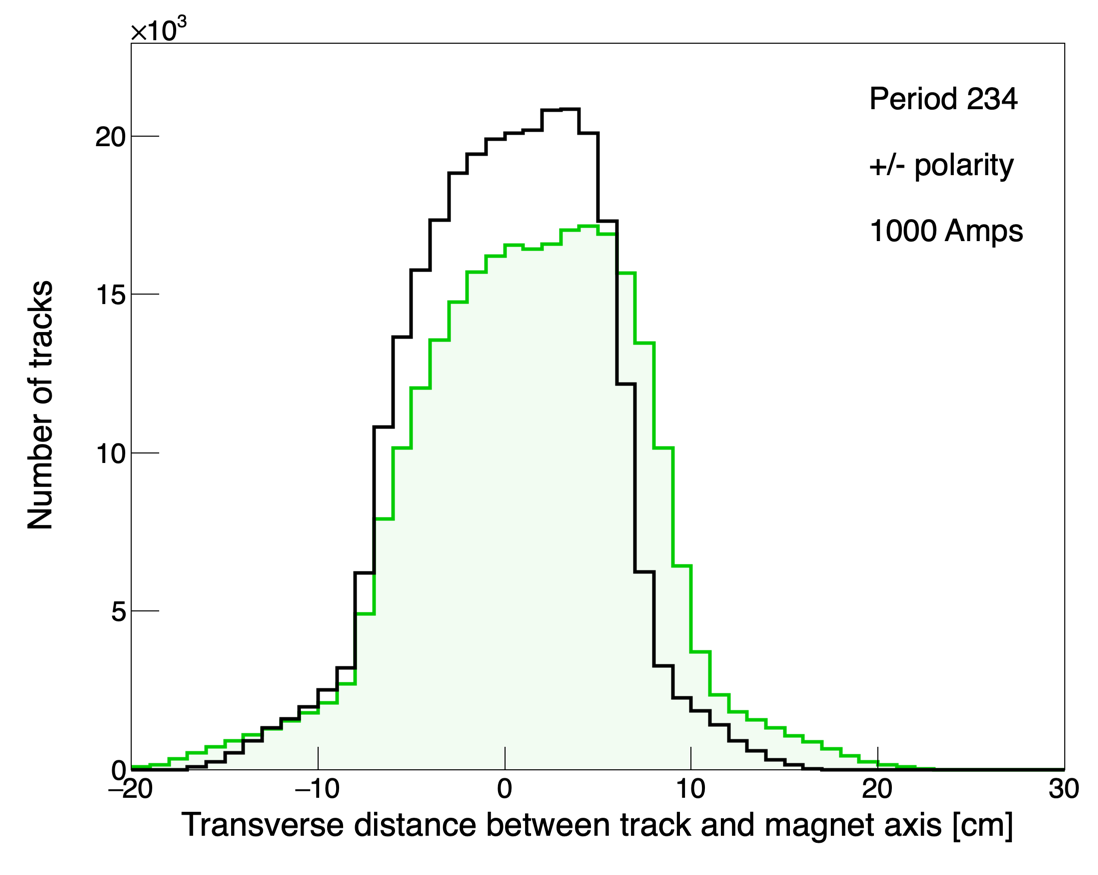
\includegraphics[width=\textwidth]{NEW-figsingle_period234_magdist_level0_posneg_stats_1000Amps.png}
            \caption{Magdist}
            \label{fig_magdist1}
           
            \end{subfigure}
            \hfill             
             \begin{subfigure}[b]{0.24\textwidth}
            \centering
	 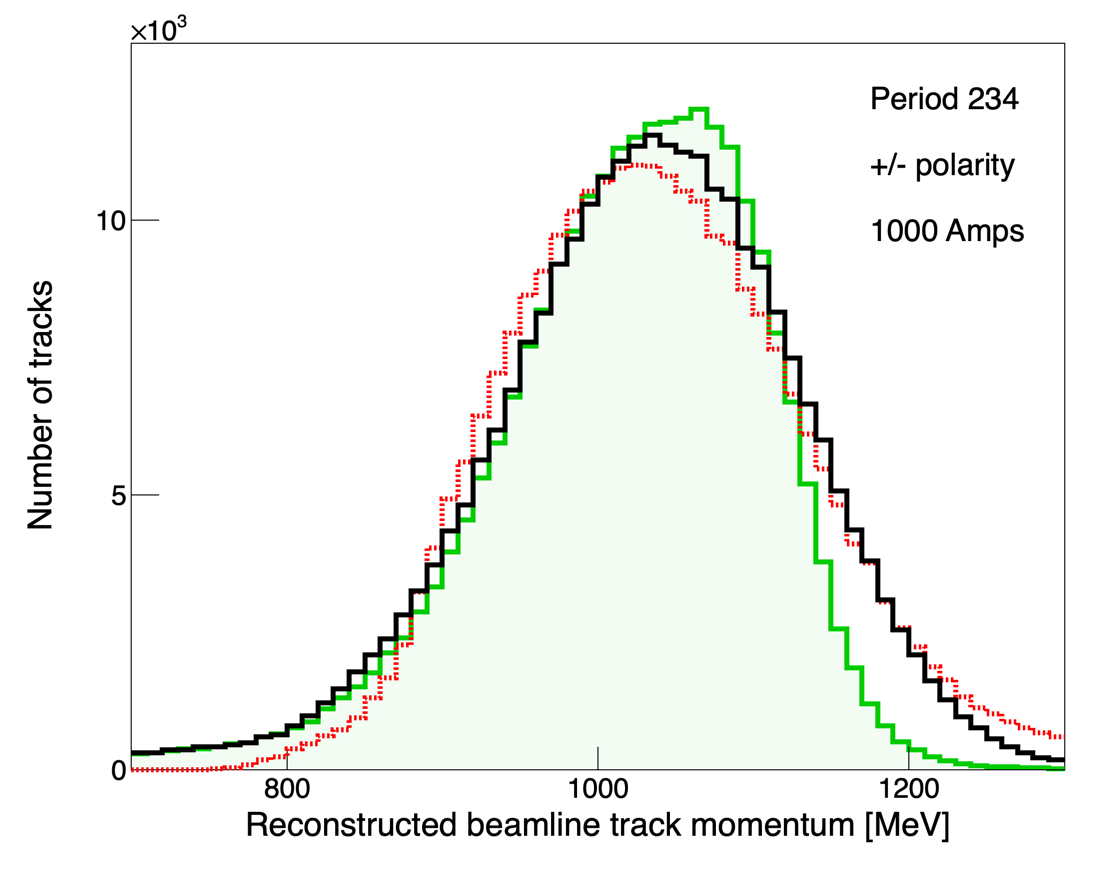
\includegraphics[width=\textwidth]{NEW-figsingle_period234_p_level0_posneg_stats_1000Amps.png}
            \caption{Momentum}
            \label{fig_p1}
            \end{subfigure}
             \hfill   
             \begin{subfigure}[b]{0.24\textwidth}
            \centering
            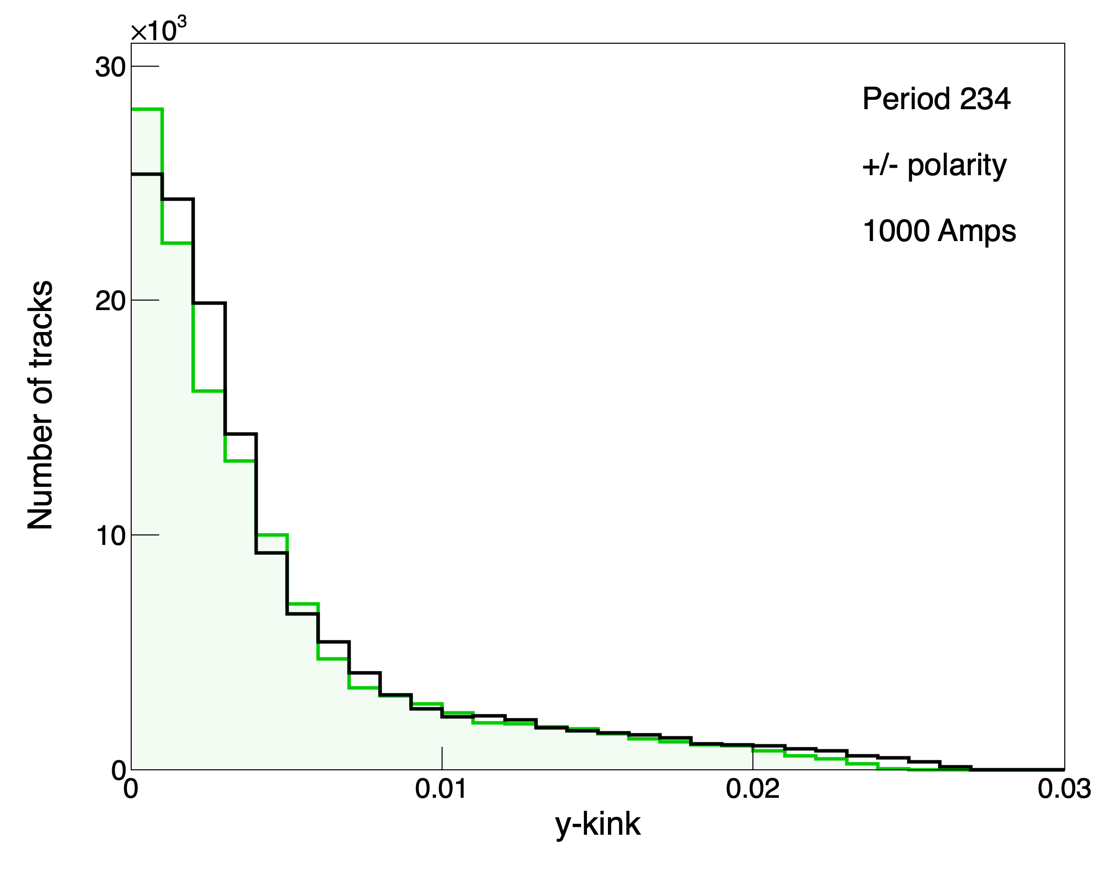
\includegraphics[width=\textwidth]{NEW-figsingle_period234_ykink_level0_posneg_stats_1000Amps.png}
            \caption{Ykink}
            \label{fig_ykink1}
            \end{subfigure}
             \hfill   
             \begin{subfigure}[b]{0.24\textwidth}
            \centering
            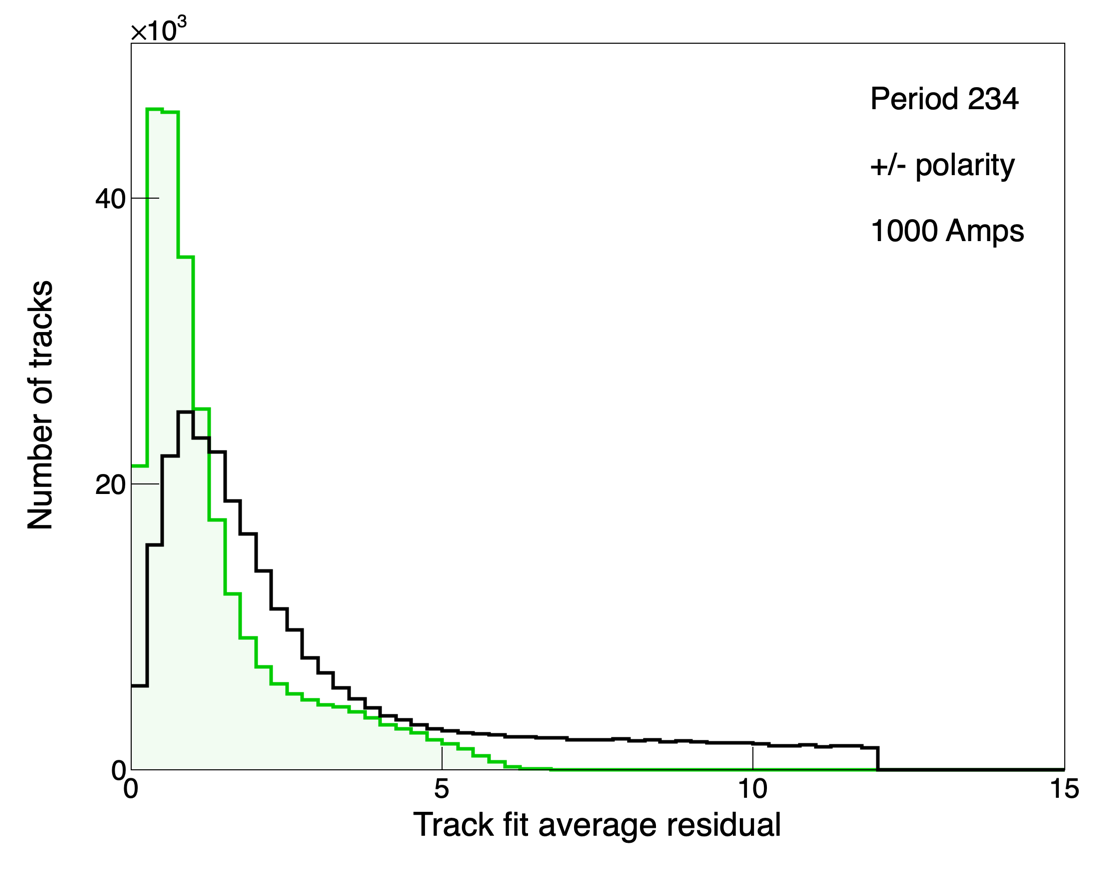
\includegraphics[width=\textwidth]{NEW-figsingle_period234_residual_level0_posneg_stats_1000Amps.png}
            \caption{Residual}
            \label{fig_residual1}
            \end{subfigure}
            
            \begin{subfigure}[b]{0.24\textwidth}
            \centering
            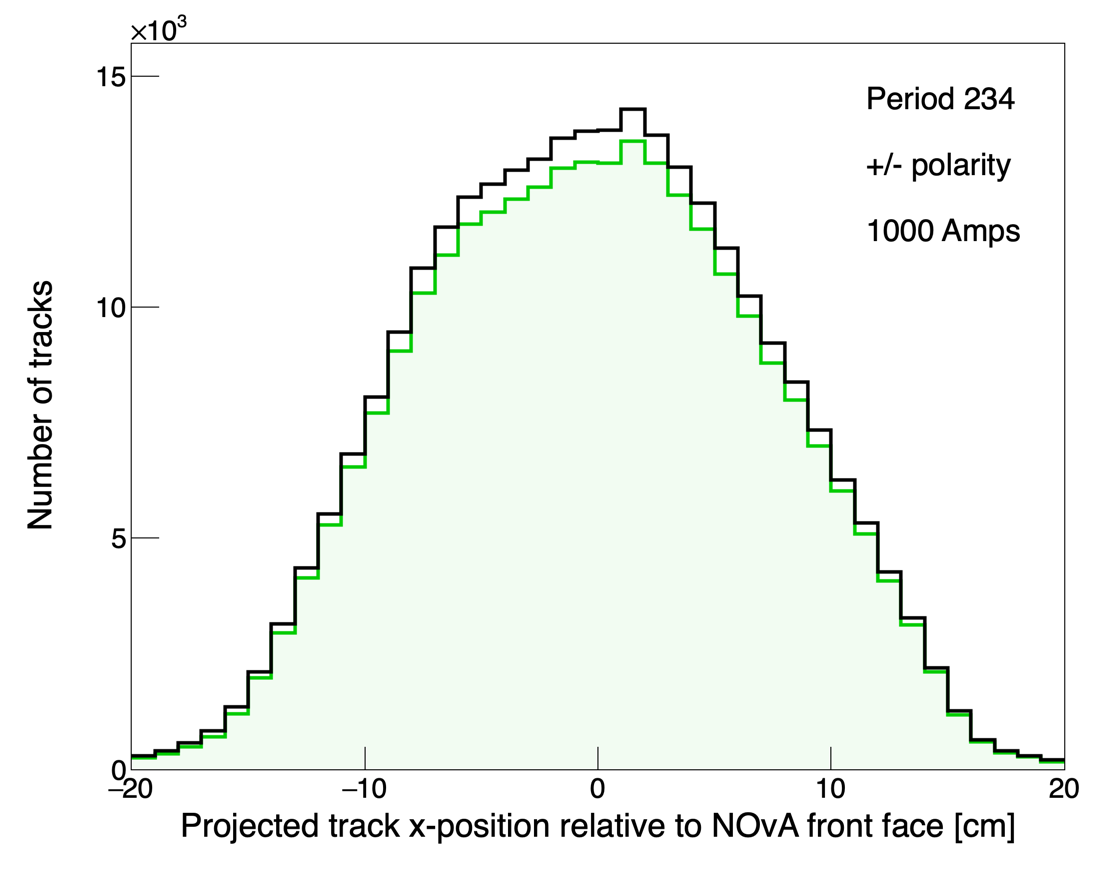
\includegraphics[width=\textwidth]{NEW-figsingle_period234_x_level0_posneg_stats_1000Amps.png}
            \caption{x}
            \label{fig_x1}
            \end{subfigure}
            \hfill             
             \begin{subfigure}[b]{0.24\textwidth}
            \centering
            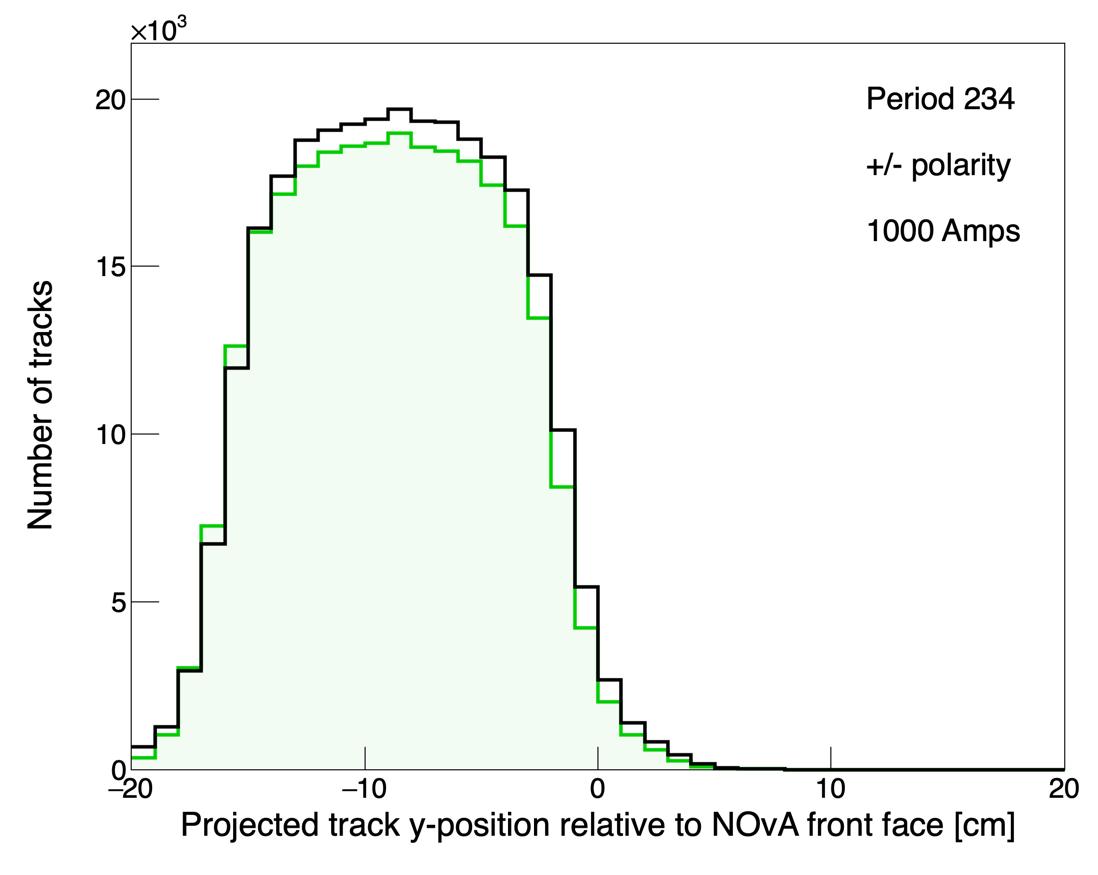
\includegraphics[width=\textwidth]{NEW-figsingle_period234_y_level0_posneg_stats_1000Amps.png}
            \caption{y}
            \label{fig_y1}
            \end{subfigure}
             \hfill   
             \begin{subfigure}[b]{0.24\textwidth}
            \centering
            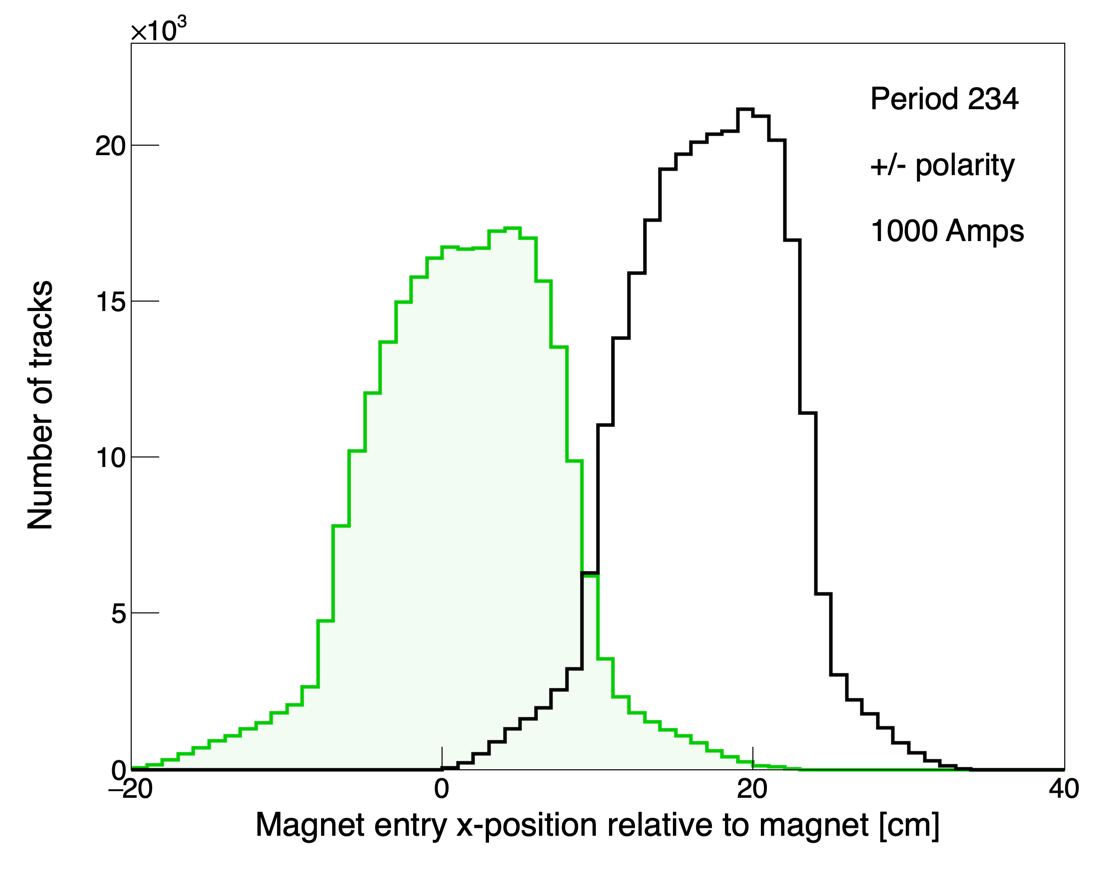
\includegraphics[width=\textwidth]{NEW-figsingle_period234_mex_level0_posneg_stats_1000Amps.png}
            \caption{mex}
            \label{fig_mex1}
            \end{subfigure}
             \hfill   
             \begin{subfigure}[b]{0.24\textwidth}
            \centering
            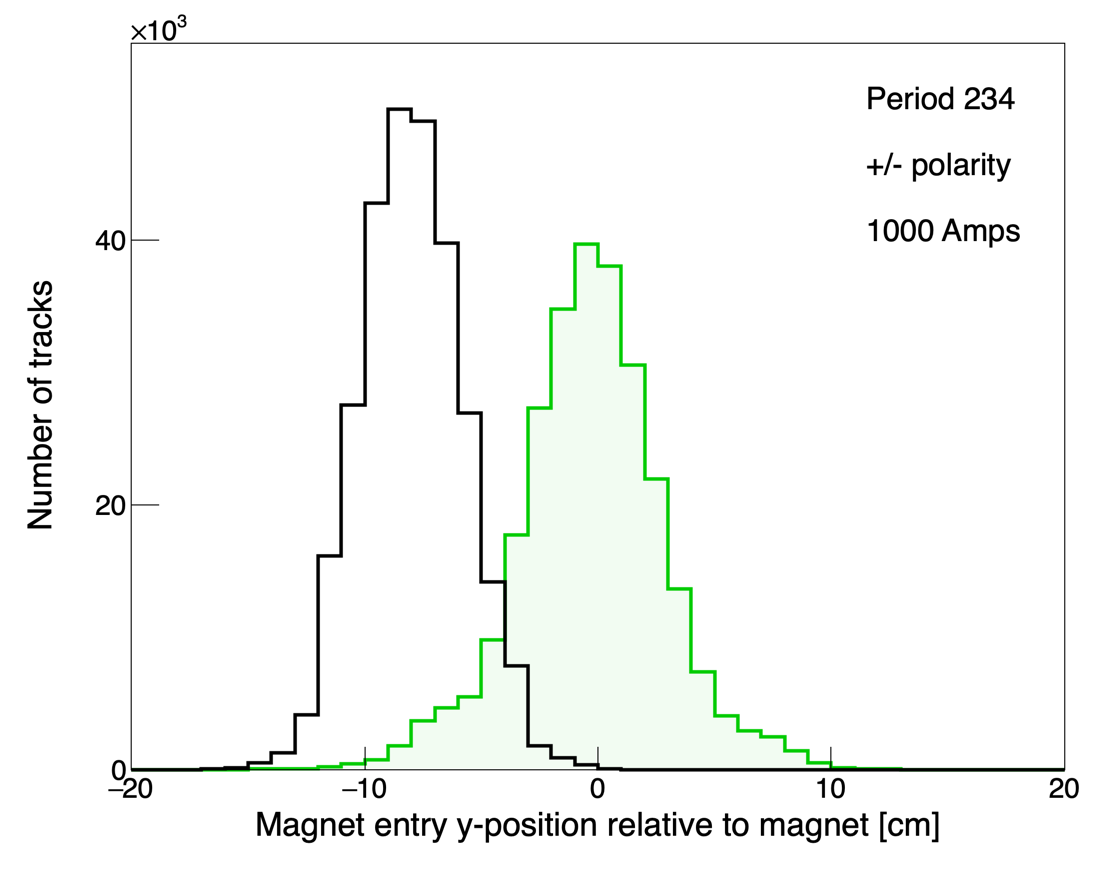
\includegraphics[width=\textwidth]{NEW-figsingle_period234_mey_level0_posneg_stats_1000Amps.png}
            \caption{mey}
            \label{fig_mey1}
            \end{subfigure}
            
            \begin{subfigure}[b]{0.24\textwidth}
            \centering
            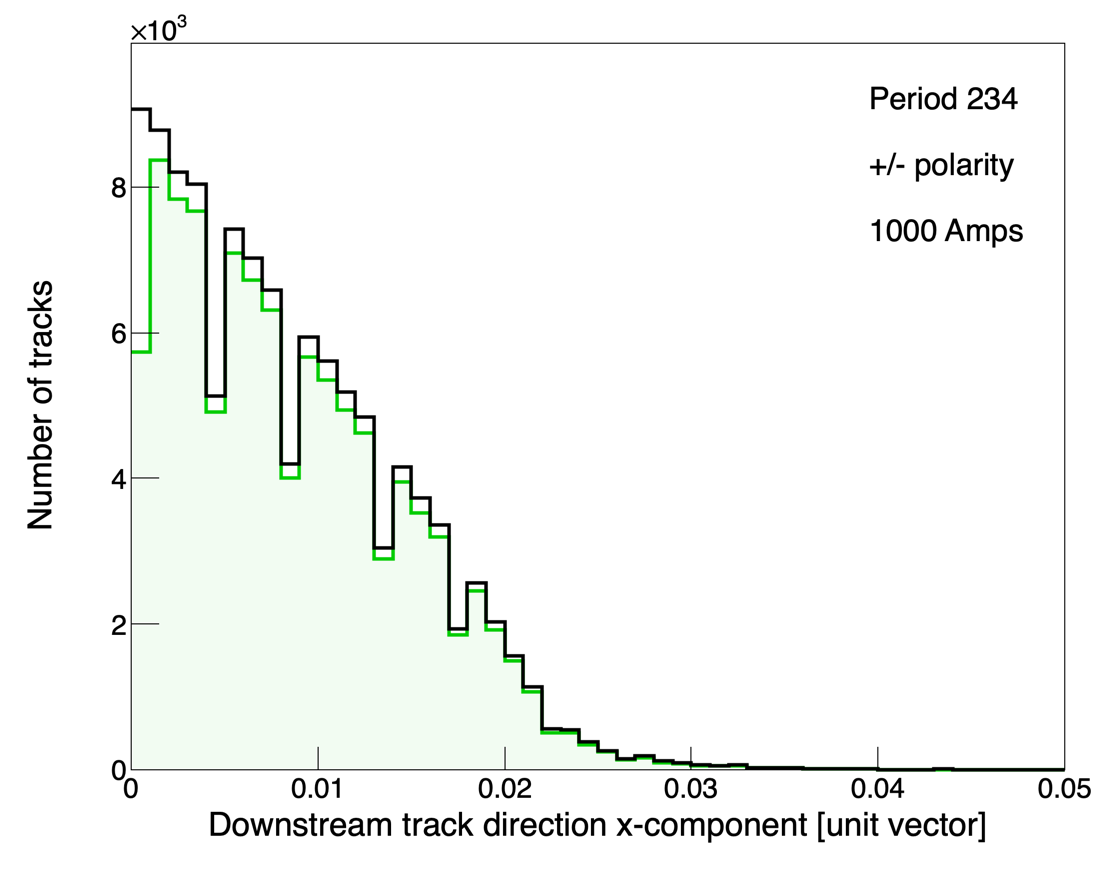
\includegraphics[width=\textwidth]{NEW-figsingle_period234_dix_level0_posneg_stats_1000Amps.png}
            \caption{dix}
            \label{fig_dix1}
            \end{subfigure}
            \hfill             
             \begin{subfigure}[b]{0.24\textwidth}
            \centering
            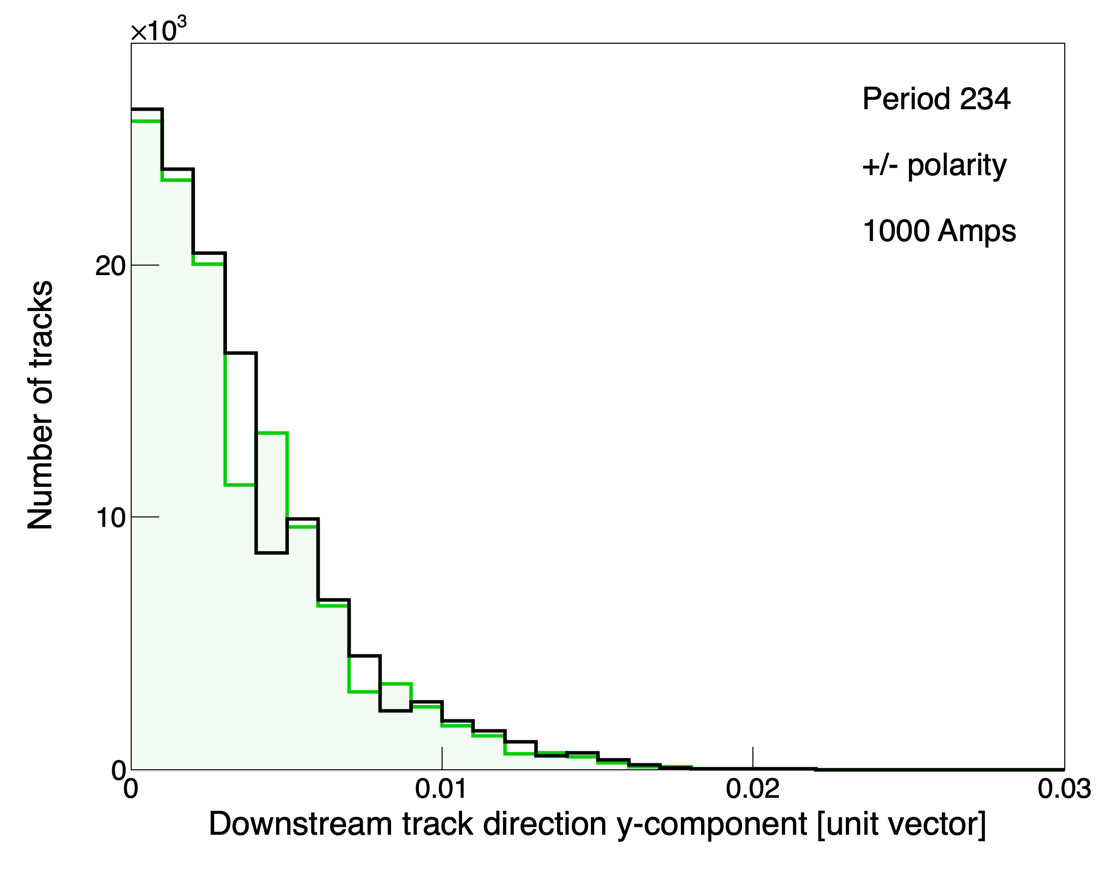
\includegraphics[width=\textwidth]{NEW-figsingle_period234_diy_level0_posneg_stats_1000Amps.png}
            \caption{diy}
            \label{fig_diy1}
            \end{subfigure}
             \hfill   
             \begin{subfigure}[b]{0.24\textwidth}
            \centering
            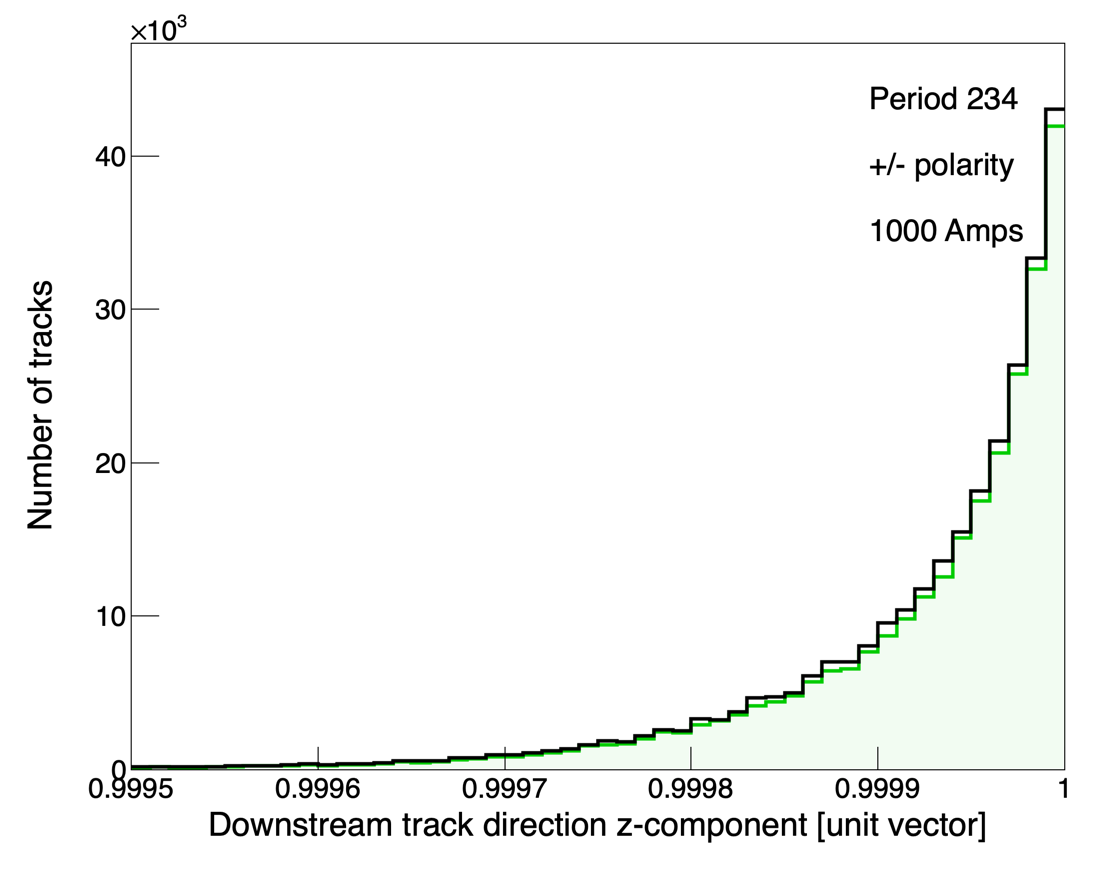
\includegraphics[width=\textwidth]{NEW-figsingle_period234_diz_level0_posneg_stats_1000Amps.png}
            \caption{diz}
            \label{fig_diz1}
            \end{subfigure}
             \hfill   
             \begin{subfigure}[b]{0.24\textwidth}
            \centering
            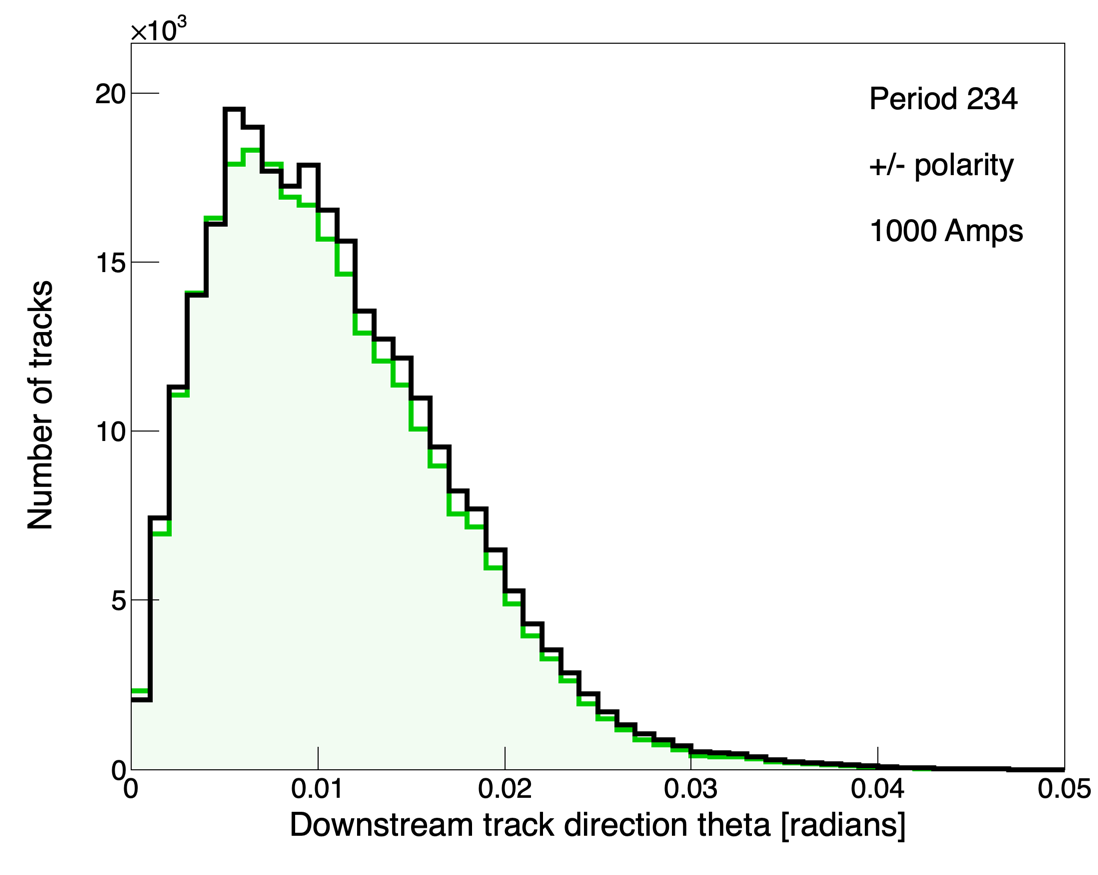
\includegraphics[width=\textwidth]{NEW-figsingle_period234_theta_level0_posneg_stats_1000Amps.png}
            \caption{theta}
            \label{fig_theta1}
            \end{subfigure}
            
            
                        \begin{subfigure}[b]{0.24\textwidth}
            \centering
            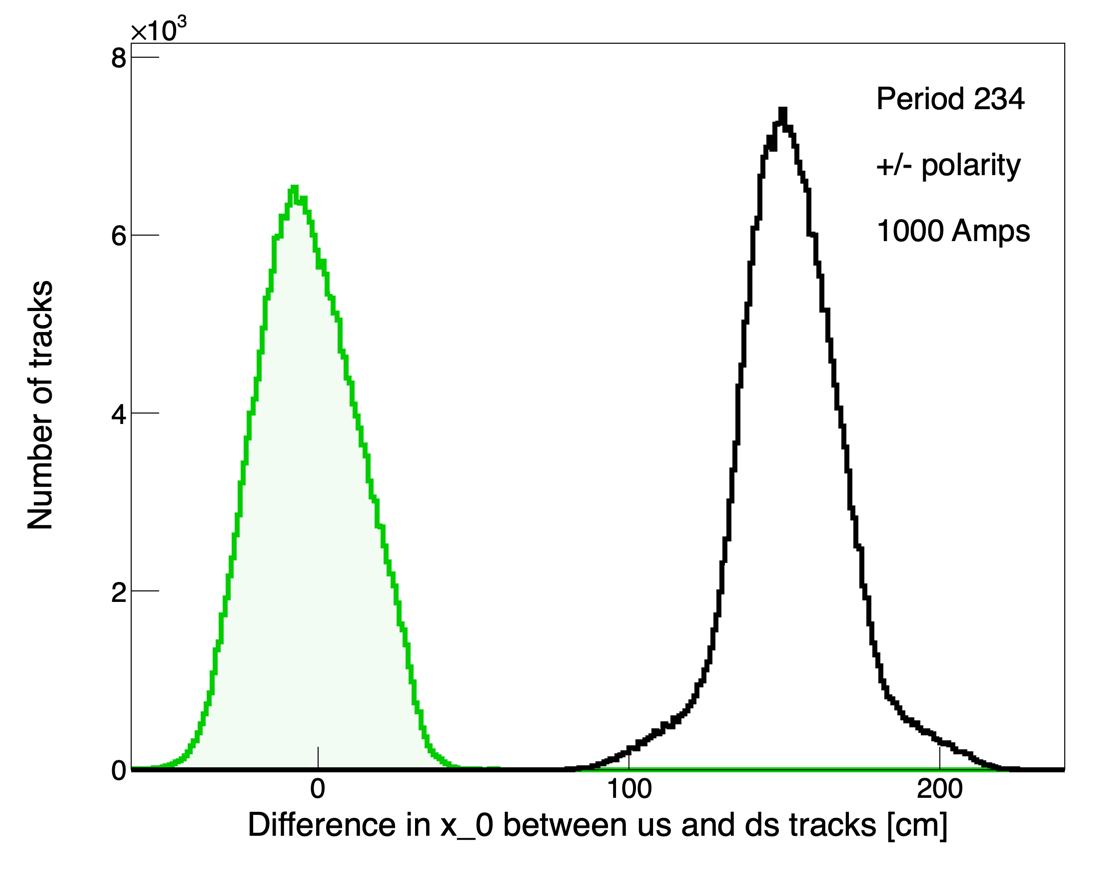
\includegraphics[width=\textwidth]{NEW-figsingle_period234_ddx_level0_posneg_stats_1000Amps.png}
            \caption{ddx}
            \label{fig_ddx1}
            \end{subfigure}
            \hfill             
             \begin{subfigure}[b]{0.24\textwidth}
            \centering
            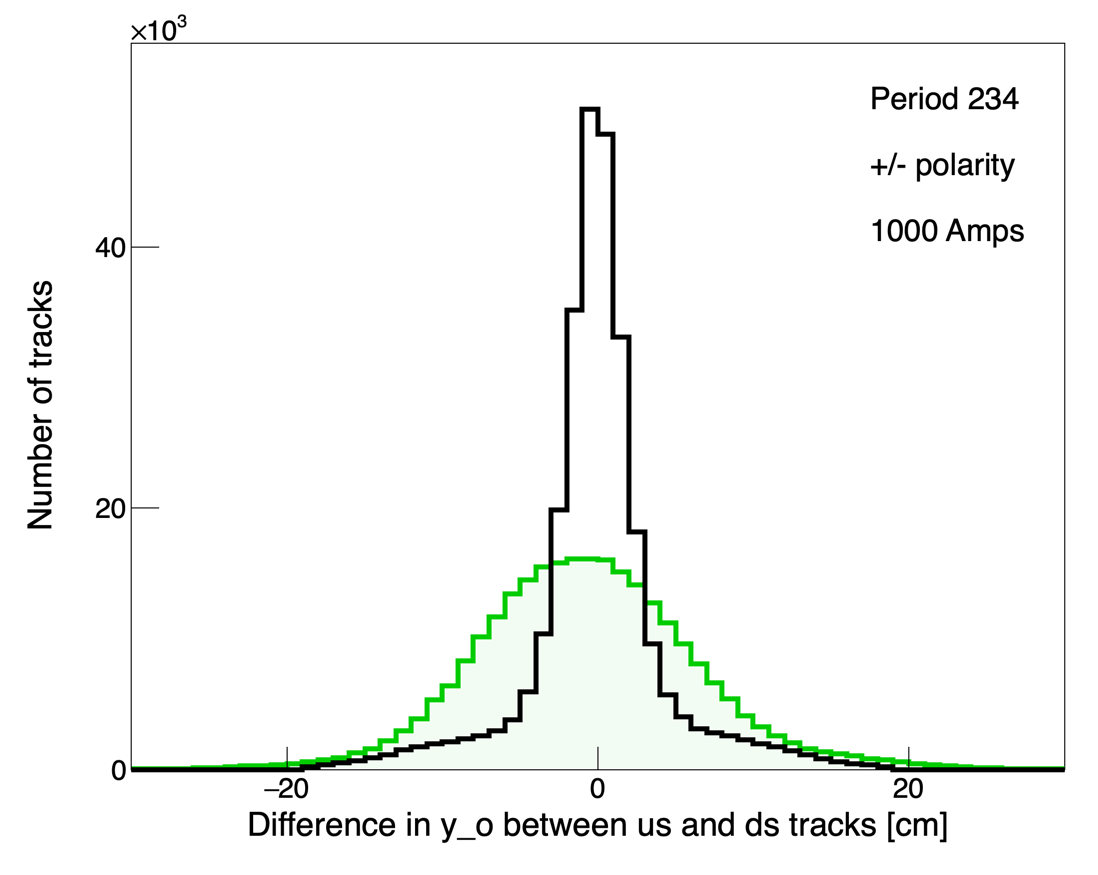
\includegraphics[width=\textwidth]{NEW-figsingle_period234_ddy_level0_posneg_stats_1000Amps.png}
            \caption{ddy}
            \label{fig_ddy1}
            \end{subfigure}
             \hfill   
             \begin{subfigure}[b]{0.24\textwidth}
            \centering
            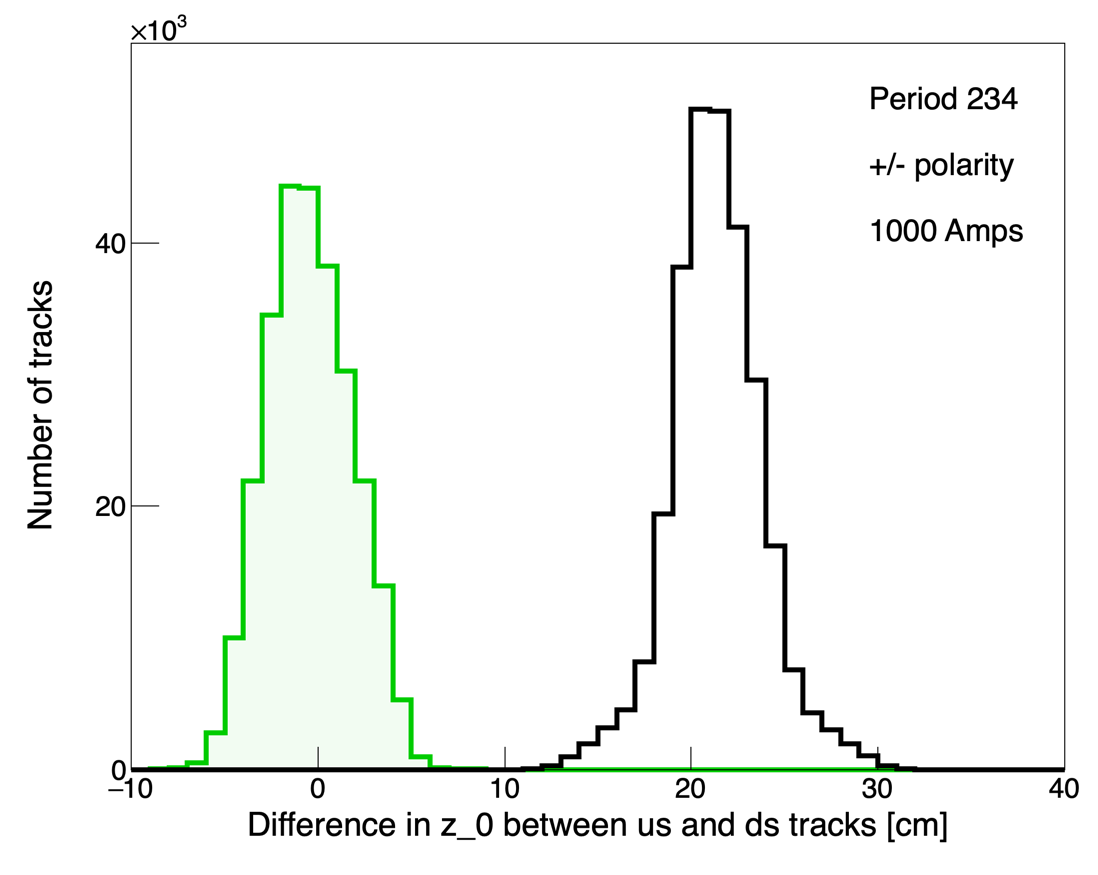
\includegraphics[width=\textwidth]{NEW-figsingle_period234_ddz_level0_posneg_stats_1000Amps.png}
            \caption{ddz}
            \label{fig_ddz1}
            \end{subfigure}
             \hfill   
             \begin{subfigure}[b]{0.24\textwidth}
            \centering
            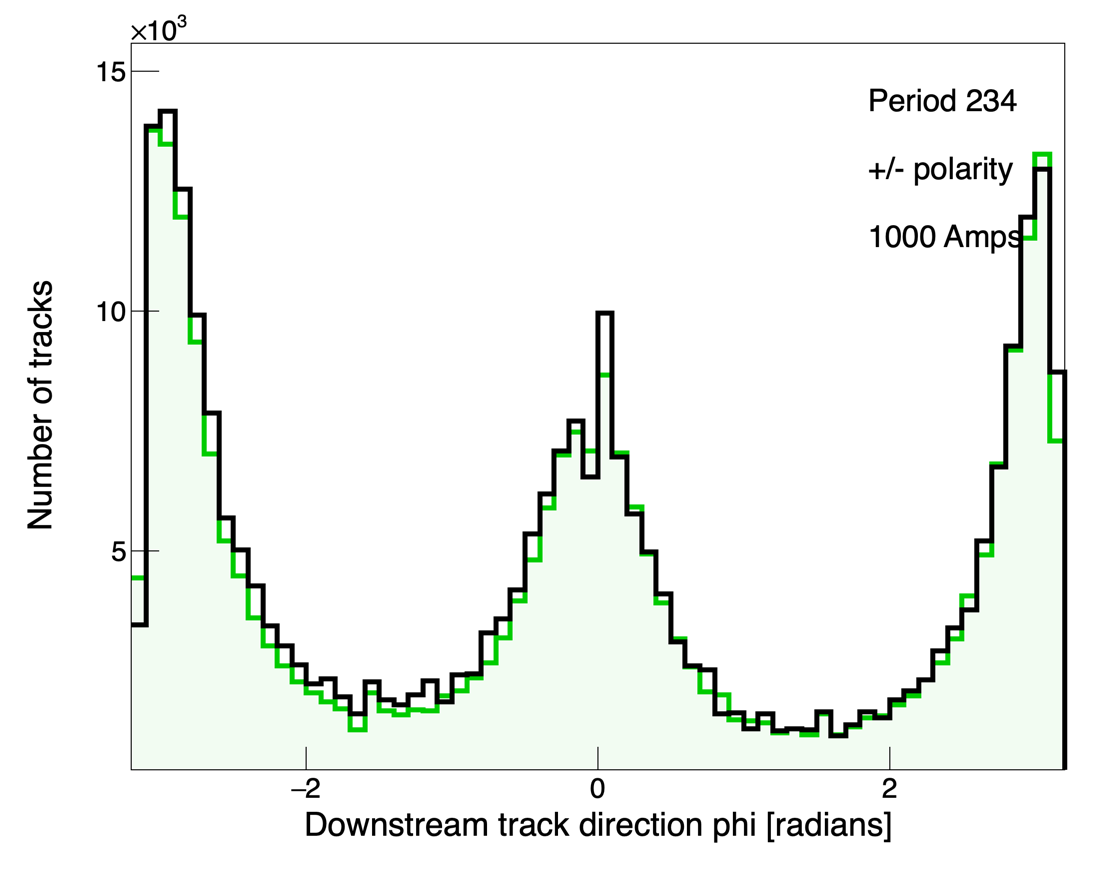
\includegraphics[width=\textwidth]{NEW-figsingle_period234_phi_level0_posneg_stats_1000Amps.png}
            \caption{phi}
            \label{fig_phi1}
            \end{subfigure}
            
            
            
   \caption[short]{The WCTrack properties.}
   \label{fig_props_overview}
  \end{figure}
  
  
  
    \newpage
  \subsection{Counting tracks of each type}
  
  First up we want to compare the counts of different types of tracks in the different regions. These counts are visualised in Table~\ref{tab_counts}. Two things to note:
  \begin{enumerate}
  \item There are notably more 3 point tracks (no wc2) in period 4 than in period 3.\\
  \item Within period 4, there are notably more 3 point tracks (no wc2) and (no wc4) when the magnet polarity is set to negative.
  \end{enumerate}
  
  
    \begin{table}[h]
        \begin{subtable}[t]{0.48\textwidth}
	\begin{center}
		\begin{tabular}{lllll}
			\toprule
			Magnet current & 500 & 750 & 1000 & 1250 \\
			\midrule
			Original Track & $\mybarr{0.061306030715445124}$ & $\mybarr{0.004370083655887127}$ & $\mybarr{1.0}$ & $\mybarr{0.0}$ \\
			New 4 point track & $\mybarr{0.05868398052191285}$ & $\mybarr{0.004370083655887127}$ & $\mybarr{0.9813959295792234}$ & $\mybarr{0.0}$ \\
			3 point (no wc2) & $\mybarr{0.014109127231864152}$ & $\mybarr{0.0011237357972281184}$ & $\mybarr{0.27456611312273693}$ & $\mybarr{0.0}$ \\
			3 point (no wc3) & $\mybarr{0.002247471594456237}$ & $\mybarr{0.0001248595330253465}$ & $\mybarr{0.03421151204894494}$ & $\mybarr{0.0}$ \\
			3 point (no wc4) & $\mybarr{0.0016231739293295043}$ & $\mybarr{0.0001248595330253465}$ & $\mybarr{0.08840054938194532}$ & $\mybarr{0.0}$ \\
			\bottomrule
		\end{tabular}
		\subcaption[]{Period 2, positive polarity. N=8009. \\[5ex] }
		\label{tab_p2_pos}
	\end{center}
        \end{subtable}
        	\hspace{\fill}
        \begin{subtable}[t]{0.48\textwidth}
	\begin{center}
		\begin{tabular}{lllll}
			\toprule
			Magnet current & 500 & 750 & 1000 & 1250 \\
			\midrule
			Original Track & $\mybarb{0.007853403141361256}$ & $\mybarb{0.0}$ & $\mybarb{1.0}$ & $\mybarb{0.0}$ \\
			New 4 point track & $\mybarb{0.007853403141361256}$ & $\mybarb{0.0}$ & $\mybarb{0.981675392670157}$ & $\mybarb{0.0}$ \\
			3 point (no wc2) & $\mybarb{0.0}$ & $\mybarb{0.0}$ & $\mybarb{0.3219895287958115}$ & $\mybarb{0.0}$ \\
			3 point (no wc3) & $\mybarb{0.0}$ & $\mybarb{0.0}$ & $\mybarb{0.034031413612565446}$ & $\mybarb{0.0}$ \\
			3 point (no wc4) & $\mybarb{0.0}$ & $\mybarb{0.0}$ & $\mybarb{0.1099476439790576}$ & $\mybarb{0.0}$ \\
			\bottomrule
		\end{tabular}
		\subcaption[]{Period 2, negative polarity. N=382. \\[5ex] }
		\label{tab_p2_pos}
	\end{center}
        \end{subtable}
        	\hspace{\fill}
	\begin{subtable}[t]{0.48\textwidth}
		\begin{tabular}{lllll}
			\toprule
			Magnet current & 500 & 750 & 1000 & 1250 \\
			\midrule
			Original Track & $\mybarr{0.6638865721434529}$ & $\mybarr{0.8090075062552127}$ & $\mybarr{1.0}$ & $\mybarr{0.0}$ \\
			New 4 point track & $\mybarr{0.6315262718932444}$ & $\mybarr{0.7753127606338616}$ & $\mybarr{0.9696413678065054}$ & $\mybarr{0.0}$ \\
			3 point (no wc2) & $\mybarr{0.07639699749791493}$ & $\mybarr{0.12543786488740616}$ & $\mybarr{0.11559633027522936}$ & $\mybarr{0.0}$ \\
			3 point (no wc3) & $\mybarr{0.022852376980817348}$ & $\mybarr{0.019683069224353627}$ & $\mybarr{0.028190158465387822}$ & $\mybarr{0.0}$ \\
			3 point (no wc4) & $\mybarr{0.030692243536280233}$ & $\mybarr{0.03319432860717264}$ & $\mybarr{0.042368640533778146}$ & $\mybarr{0.0}$ \\
			\bottomrule
		\end{tabular}
		\subcaption[]{Period 3, positive polarity. N=5995. \\[5ex] }
		\label{tab_p3_pos}
	\end{subtable}
	\hspace{\fill}
		\begin{subtable}[t]{0.48\textwidth}
		\begin{tabular}{lllll}
			\toprule
			Magnet current & 500 & 750 & 1000 & 1250 \\
			\midrule
			Original Track & $\mybarb{0.014246575342465753}$ & $\mybarb{1.0}$ & $\mybarb{0.021369863013698632}$ & $\mybarb{0.0}$ \\
			New 4 point track & $\mybarb{0.01315068493150685}$ & $\mybarb{0.9627397260273972}$ & $\mybarb{0.021369863013698632}$ & $\mybarb{0.0}$ \\
			3 point (no wc2) & $\mybarb{0.0032876712328767125}$ & $\mybarb{0.08493150684931507}$ & $\mybarb{0.002191780821917808}$ & $\mybarb{0.0}$ \\
			3 point (no wc3) & $\mybarb{0.0}$ & $\mybarb{0.024657534246575342}$ & $\mybarb{0.0027397260273972603}$ & $\mybarb{0.0}$ \\
			3 point (no wc4) & $\mybarb{0.001095890410958904}$ & $\mybarb{0.03561643835616438}$ & $\mybarb{0.0016438356164383563}$ & $\mybarb{0.0}$ \\
			\bottomrule
		\end{tabular}
		\subcaption[]{Period 3, negative polarity. N=1825.\\[5ex]}
		\label{tab_p3_neg}
	\end{subtable}
	\hspace{\fill}
	\begin{subtable}[t]{0.48\textwidth}
		\begin{tabular}{lllll}
			\toprule
			Magnet current & 500 & 750 & 1000 & 1250 \\
			\midrule
			Original Track & $\mybarr{0.11053355756000612}$ & $\mybarr{0.49006268154716404}$ & $\mybarr{1.0}$ & $\mybarr{0.22320746063293073}$ \\
			New 4 point track & $\mybarr{0.10250726188656169}$ & $\mybarr{0.4697293991744382}$ & $\mybarr{0.9665188809050604}$ & $\mybarr{0.21434031493655403}$ \\
			3 point (no wc2) & $\mybarr{0.08293838862559241}$ & $\mybarr{0.30110074912092955}$ & $\mybarr{0.24690414309738573}$ & $\mybarr{0.19912857361259748}$ \\
			3 point (no wc3) & $\mybarr{0.005733068338174591}$ & $\mybarr{0.025454823421495184}$ & $\mybarr{0.08087448402384956}$ & $\mybarr{0.005503745604647607}$ \\
			3 point (no wc4) & $\mybarr{0.03462773276257453}$ & $\mybarr{0.08546093869438924}$ & $\mybarr{0.04915150588595016}$ & $\mybarr{0.06314019263109616}$ \\
			\bottomrule
		\end{tabular}
		\subcaption[]{Period 4, positive polarity. N=13082. }
		\label{tab_p4_pos}
	\end{subtable}
	\hspace{\fill}
	\begin{subtable}[t]{0.48\textwidth}
		\begin{tabular}{lllll}
			\toprule
			Magnet current & 500 & 750 & 1000 & 1250 \\
			\midrule
			Original Track & $\mybarb{0.47055555555555556}$ & $\mybarb{0.5969444444444445}$ & $\mybarb{0.8247222222222222}$ & $\mybarb{0.3113888888888889}$ \\
			New 4 point track & $\mybarb{0.44333333333333336}$ & $\mybarb{0.565}$ & $\mybarb{0.7808333333333334}$ & $\mybarb{0.3}$ \\
			3 point (no wc2) & $\mybarb{0.36277777777777775}$ & $\mybarb{0.69}$ & $\mybarb{1.0}$ & $\mybarb{0.2927777777777778}$ \\
			3 point (no wc3) & $\mybarb{0.026944444444444444}$ & $\mybarb{0.0525}$ & $\mybarb{0.06444444444444444}$ & $\mybarb{0.0175}$ \\
			3 point (no wc4) & $\mybarb{0.16416666666666666}$ & $\mybarb{0.20527777777777778}$ & $\mybarb{0.29638888888888887}$ & $\mybarb{0.09722222222222222}$ \\
			\bottomrule
		\end{tabular}
		\subcaption[]{Period 4, negative polarity. N=3600.}
		\label{tab_p4_neg}
	\end{subtable}
	\caption[]{Counts for the different track types sub-divided by data taking period, magnet polarity, and magnet current in Amps. The maximum data bar scale in each case is given by N = number of tracks.}
	\label{tab_counts}
\end{table}

  
The reader may find it easier to visualise using Figure~\ref{fig_momentum}.

  \begin{figure}[h]
    \centering   
     	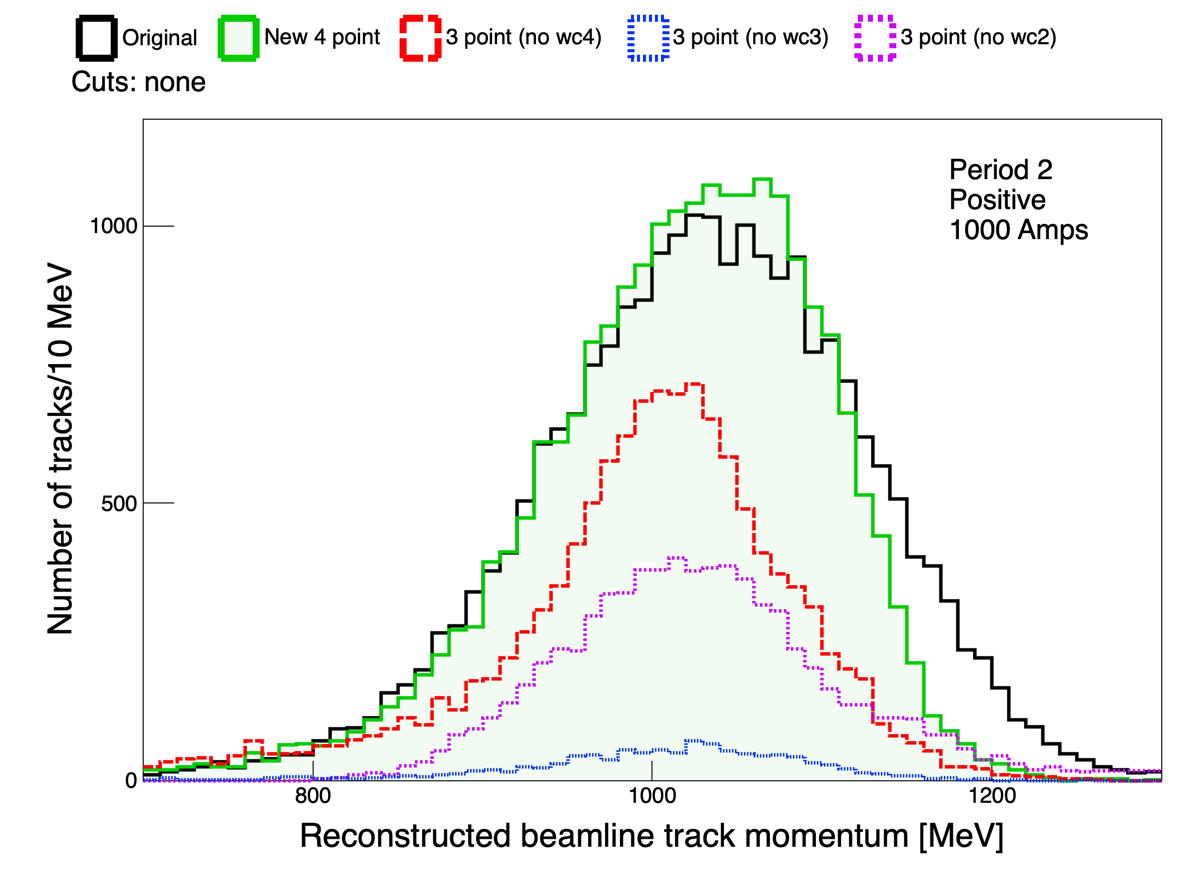
\includegraphics[scale=0.18]{NEW-figsingle_period2_p_level0_pos_stats_1000Amps.png}
	 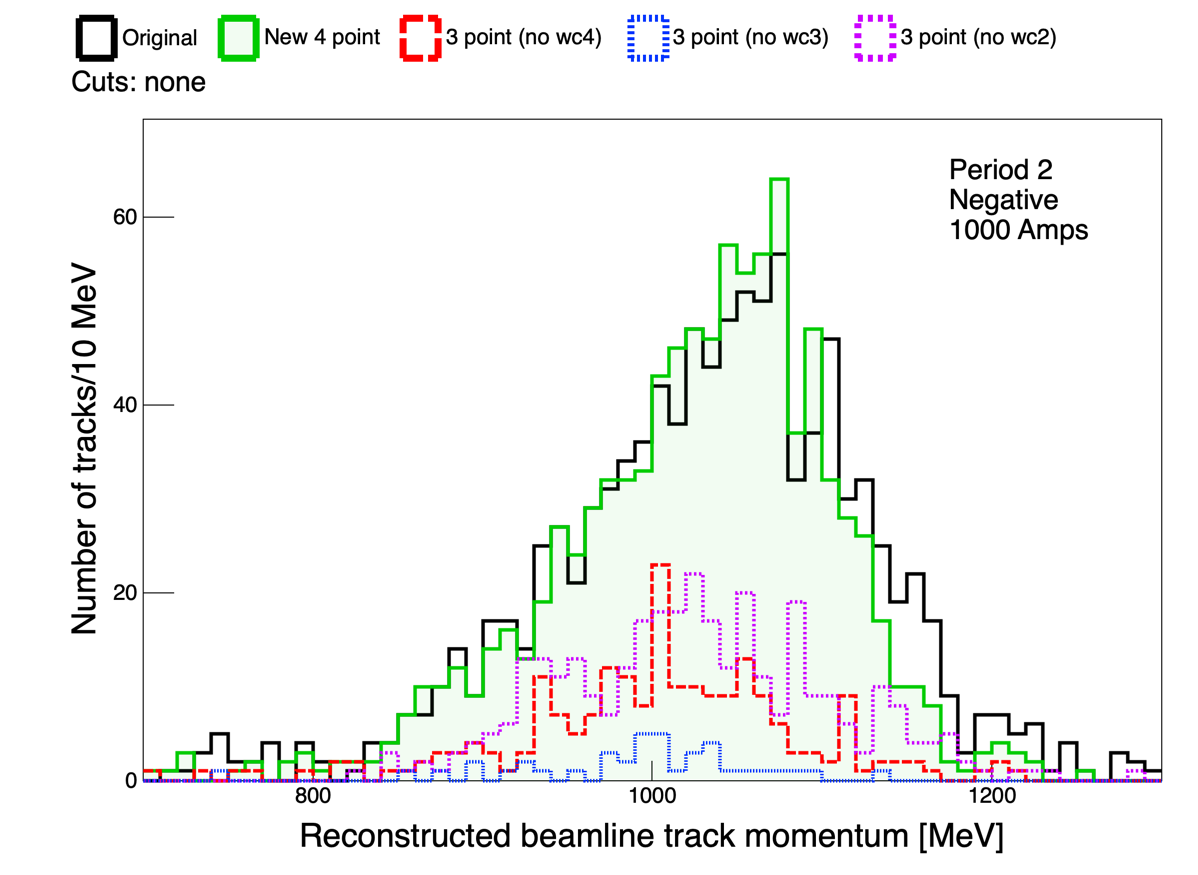
\includegraphics[scale=0.18]{NEW-figsingle_period2_p_level0_neg_stats_1000Amps.png}
	 
   	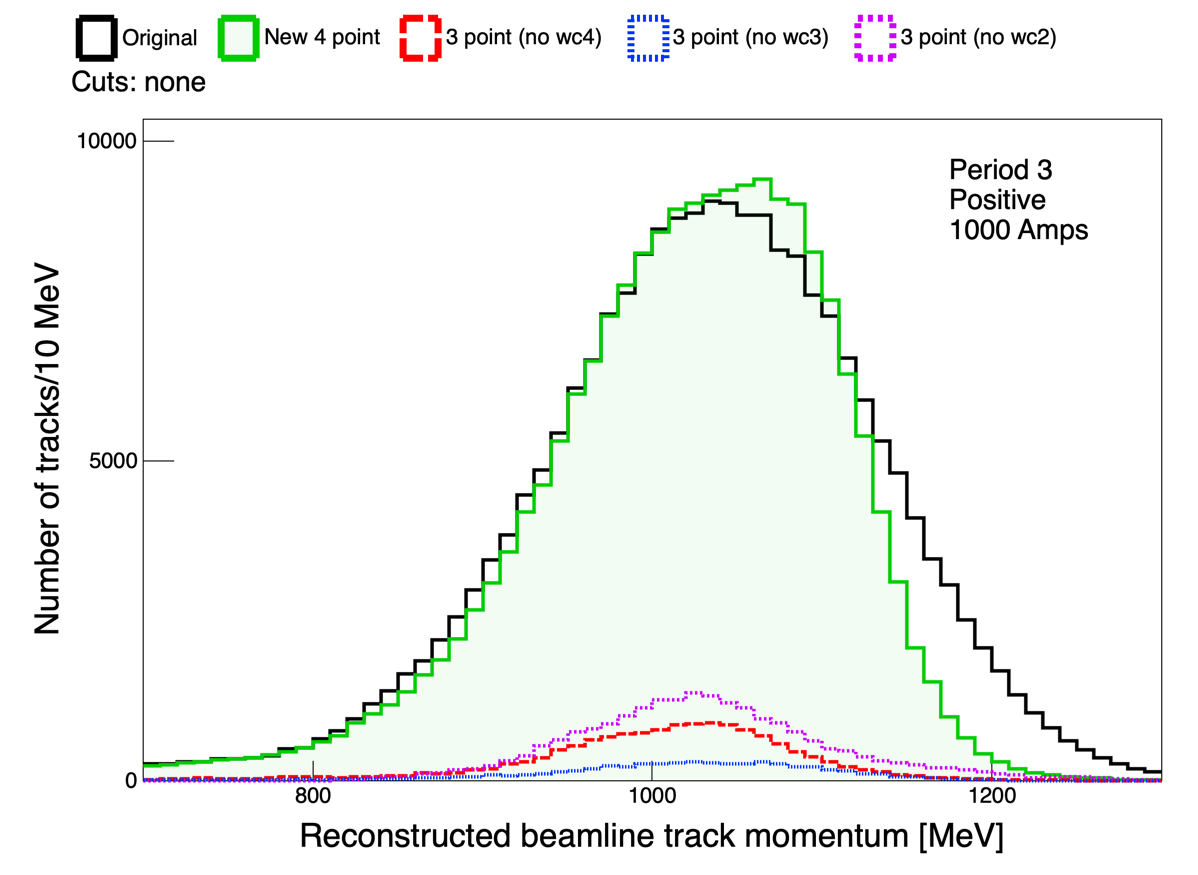
\includegraphics[scale=0.18]{NEW-figsingle_period3_p_level0_pos_stats_1000Amps.png}
	 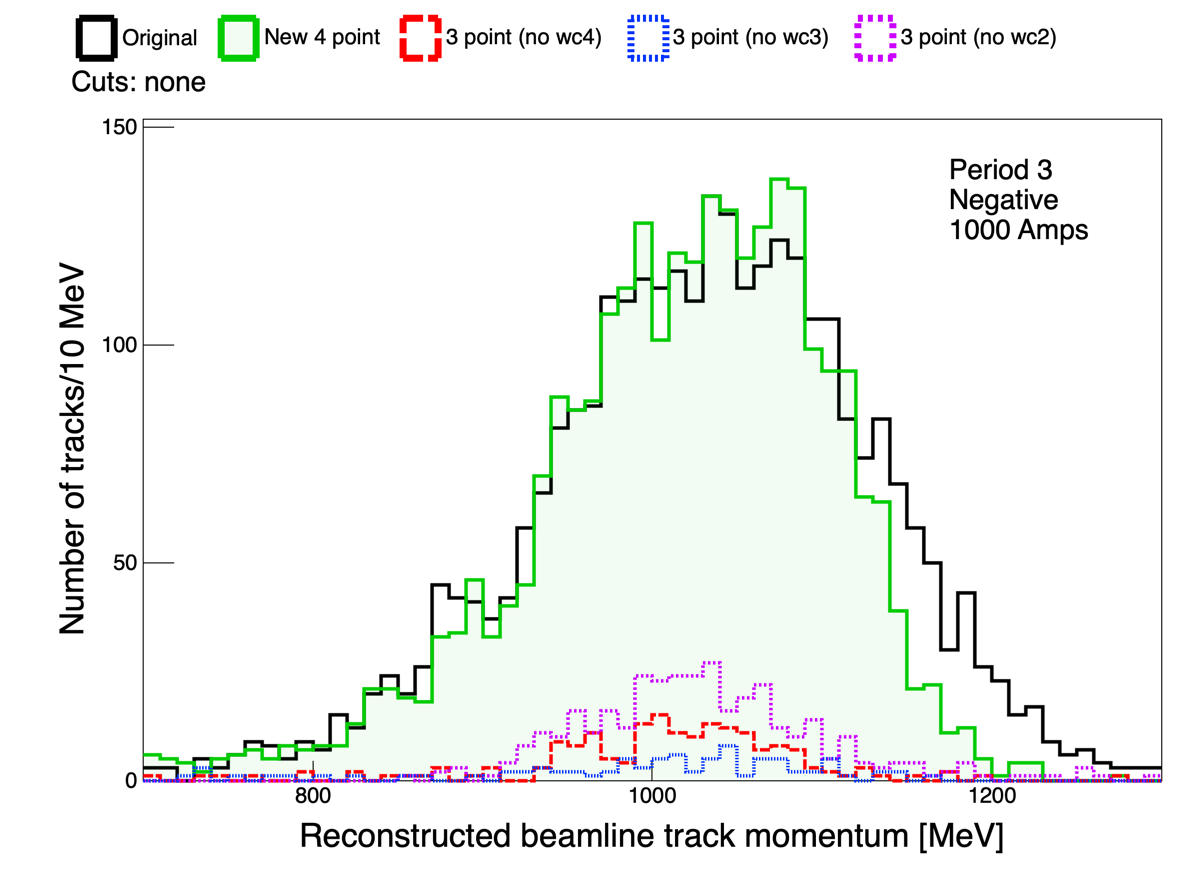
\includegraphics[scale=0.18]{NEW-figsingle_period3_p_level0_neg_stats_1000Amps.png}
	 
 	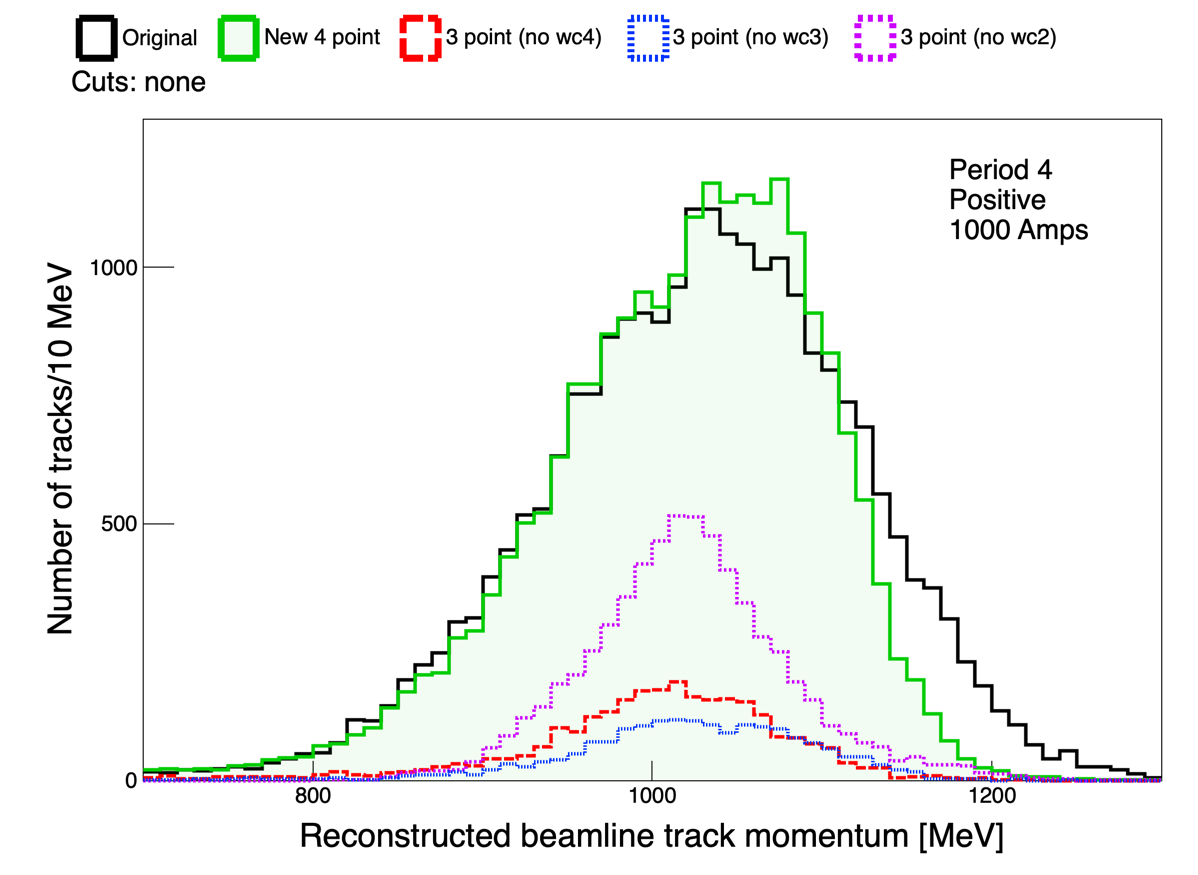
\includegraphics[scale=0.18]{NEW-figsingle_period4_p_level0_pos_stats_1000Amps.png}
	 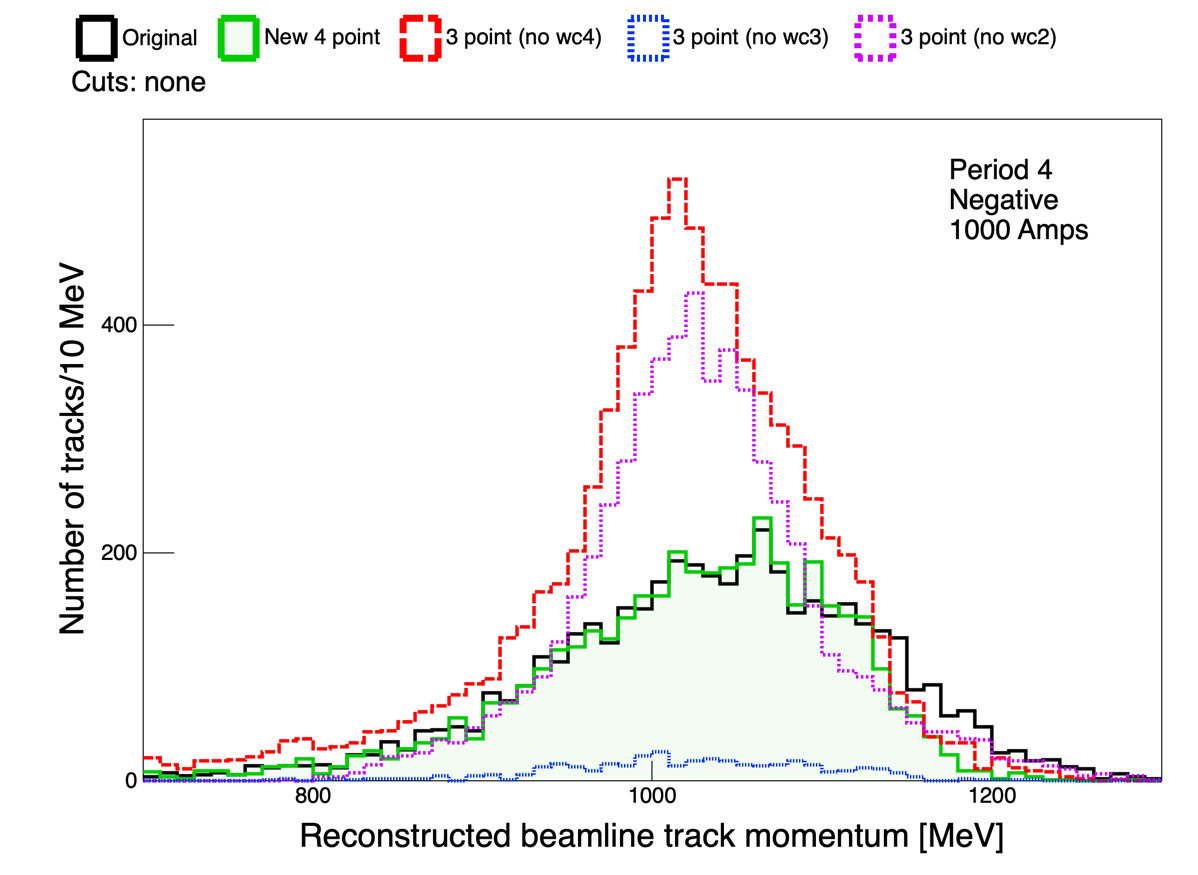
\includegraphics[scale=0.18]{NEW-figsingle_period4_p_level0_neg_stats_1000Amps.png}
   \caption[short]{The WCTrack momentum with magnet current 1000 Amps. Left: positive polarity, Right: negative polarity, Top: period 3, Bottom: period 4. No cuts applied.}
   \label{fig_momentum}
  \end{figure}
 
 
 Figure~\ref{fig_intensity} and  Figure~\ref{fig_run} show the intensity and run number distributions.
  
When the magnet polarity is set to negative, only negatively charged particles (predominantly pions) are permitted to continue through the magnetic field region in the direction of the downstream wirechambers 3 and 4 and baby NOvA. There is no reason I can think of that would make a change in the magnet's polarity result in wirechamber 2 or 4 being less efficient. The negative polarity runs were not grouped together in time (if they were, one might suspect a degrading performance of WC over time).

My plan to explore this further was to make plots of the hit positions within each wire chamber for negative and positive polarity; these are shown in Figure~\ref{fig_xyhitspol} and don't indicate any polarity-related differences between the wirechambers' performance. So I went back to thinking about what other conditions were related to the polarity differences.

\textcolor{red}{I concluded that there is no correlation between polarity and WC performance - gave a talk on it late April. add a para on that.}


  \begin{figure}[h]
    \centering   
     	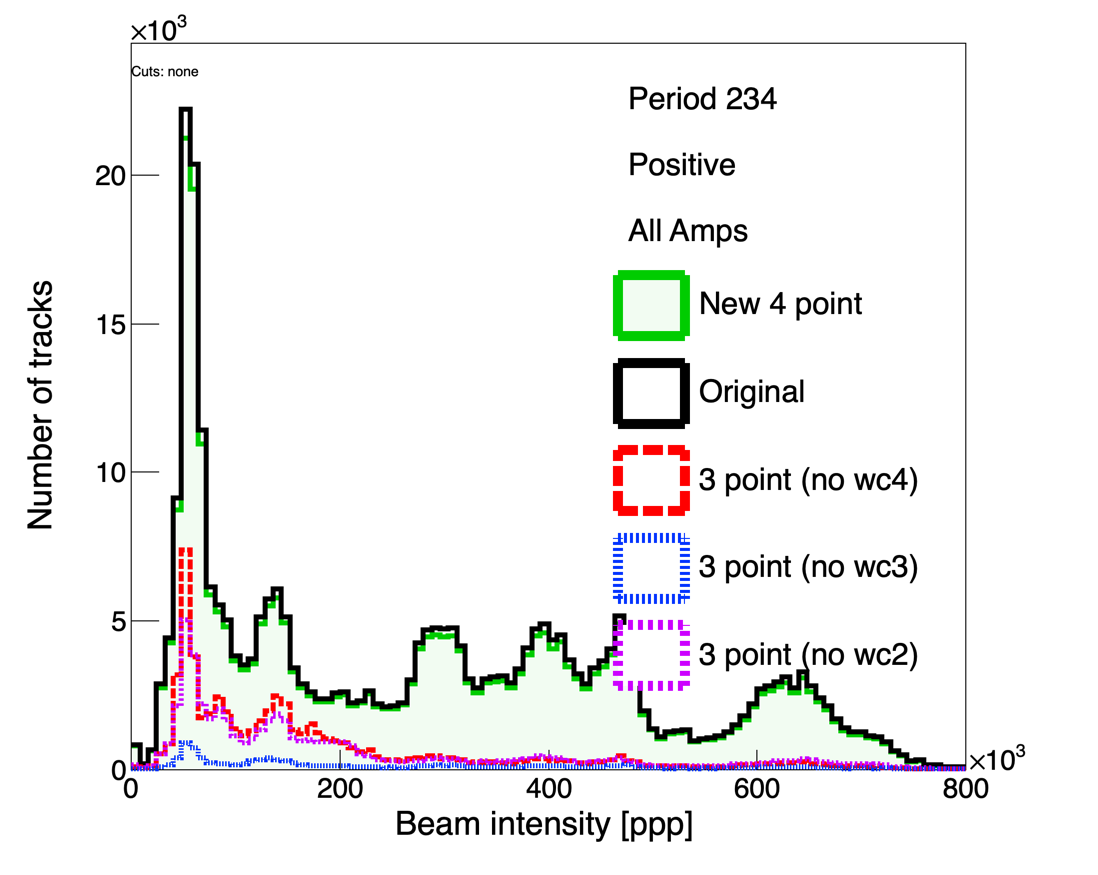
\includegraphics[scale=0.18]{NEW-figsingle_period234_intensity_level0_pos_stats_allAmps_nomomcut.png}
	 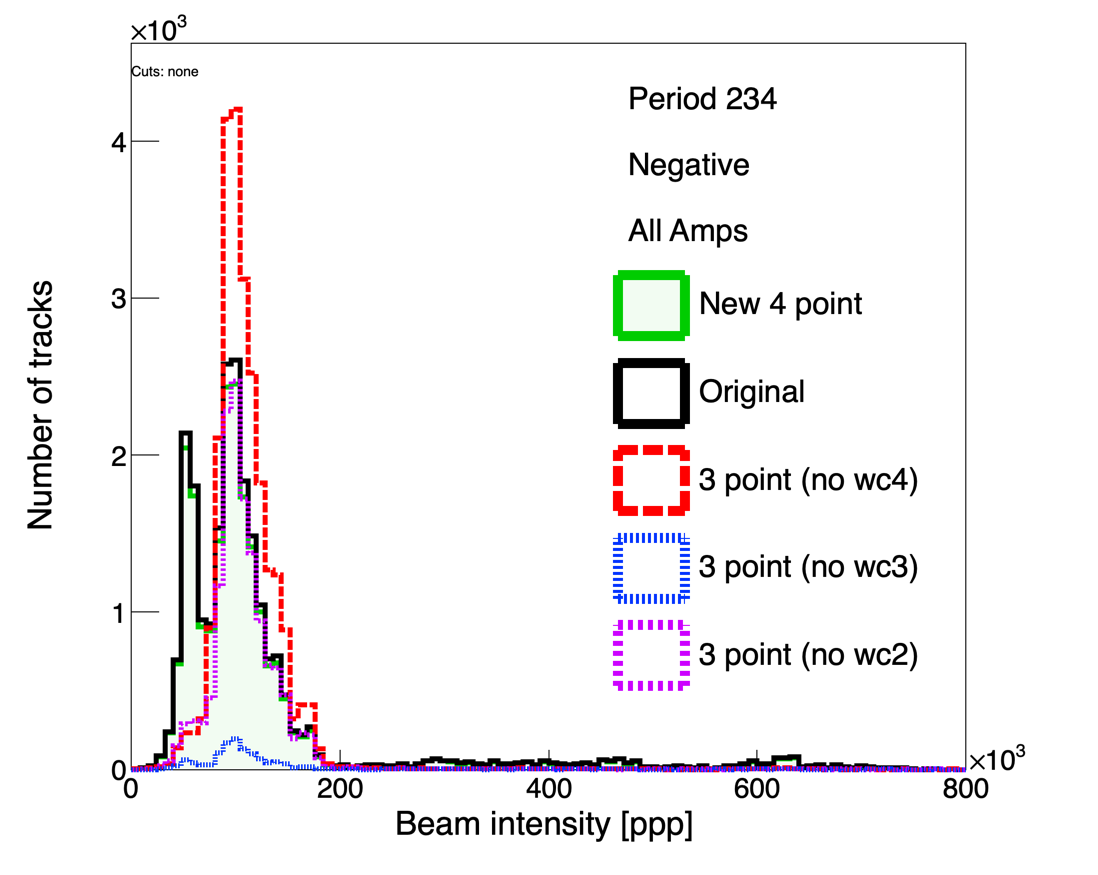
\includegraphics[scale=0.18]{NEW-figsingle_period234_intensity_level0_neg_stats_allAmps_nomomcut.png}
	 
   	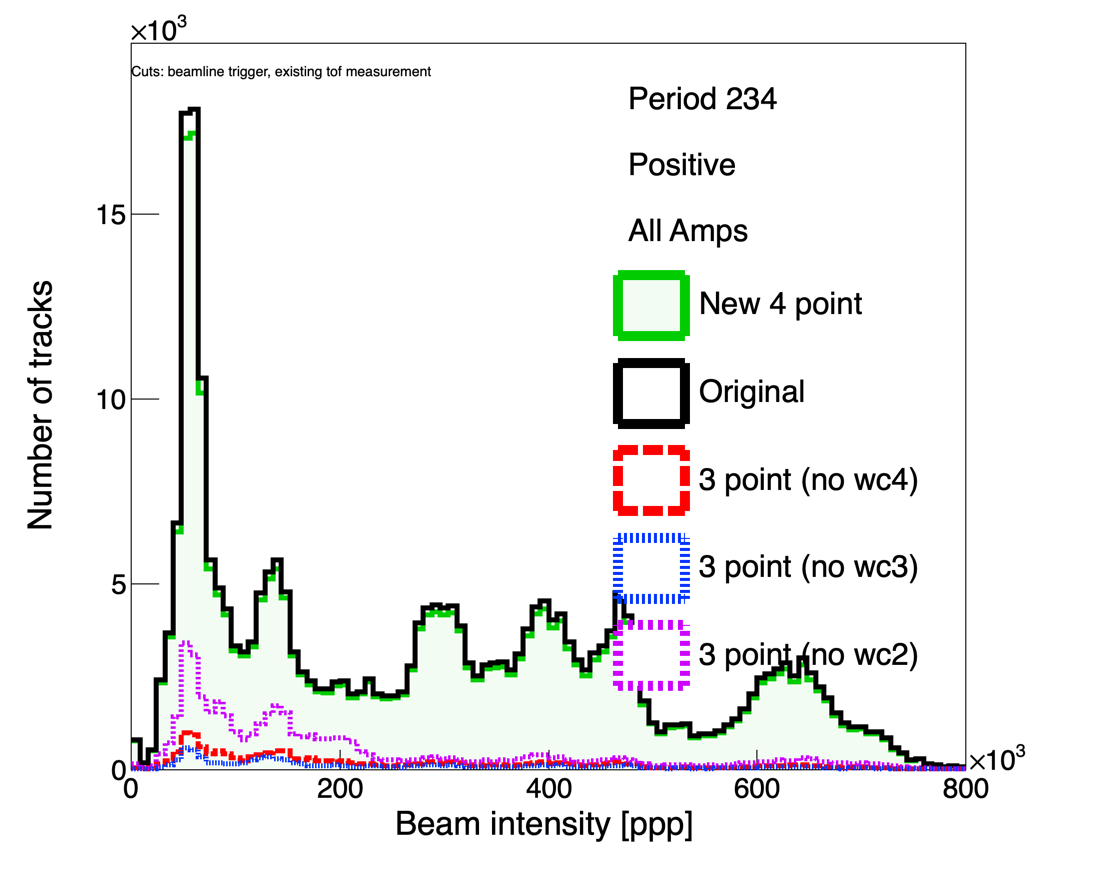
\includegraphics[scale=0.18]{NEW-figsingle_period234_intensity_level2_pos_stats_allAmps_nomomcut.png}
	 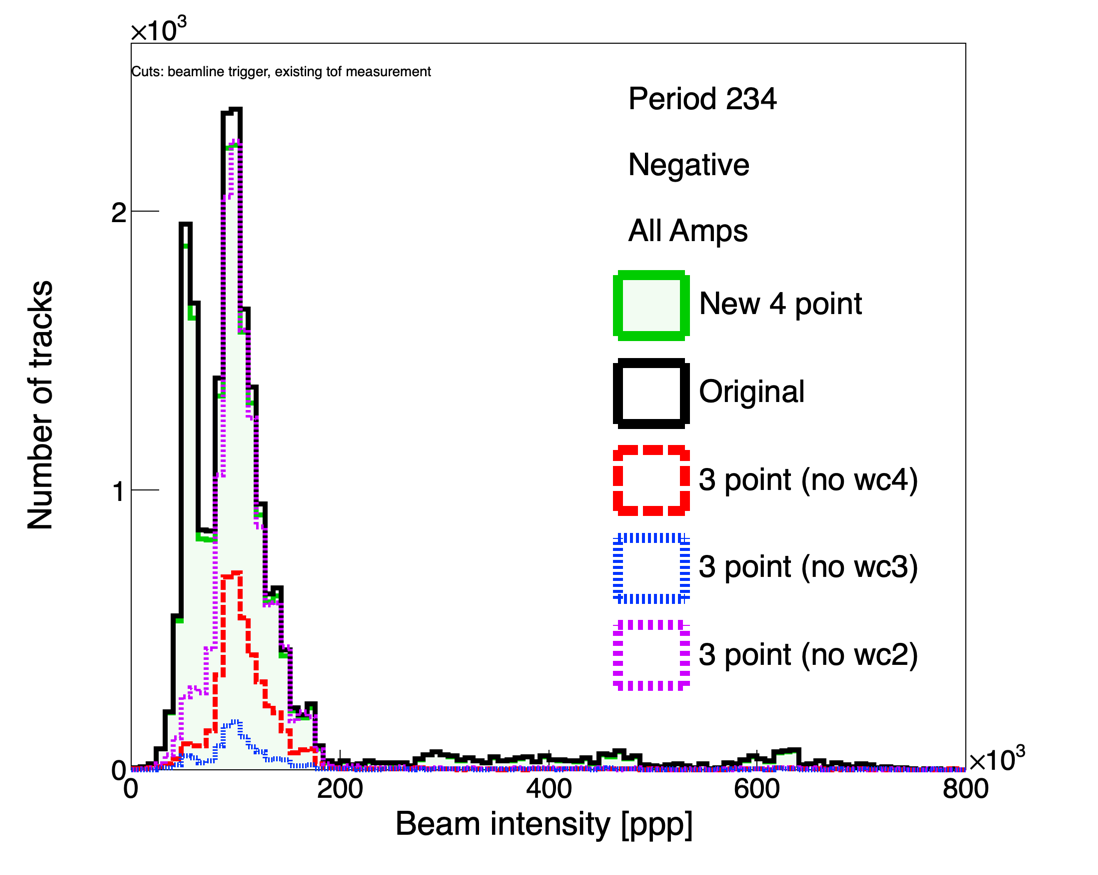
\includegraphics[scale=0.18]{NEW-figsingle_period234_intensity_level2_neg_stats_allAmps_nomomcut.png}
	 
 	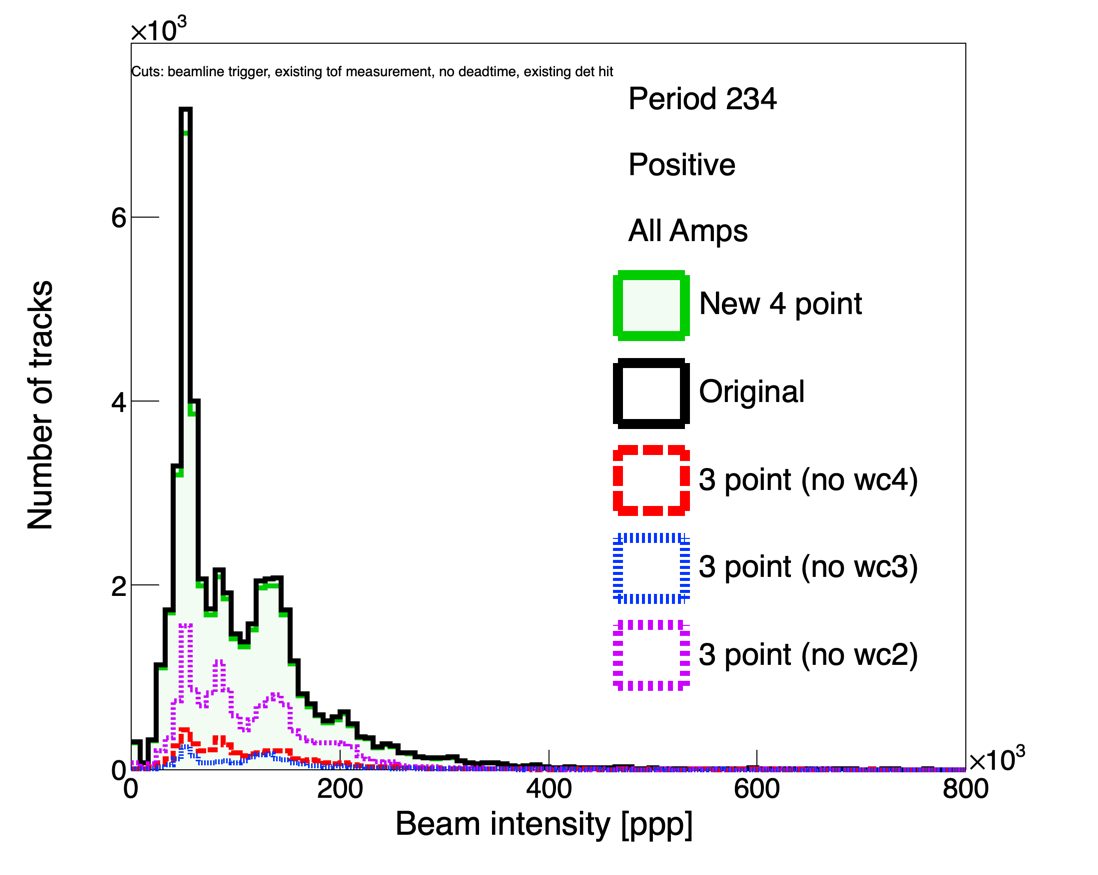
\includegraphics[scale=0.18]{NEW-figsingle_period234_intensity_level4_pos_stats_allAmps_nomomcut.png}
	 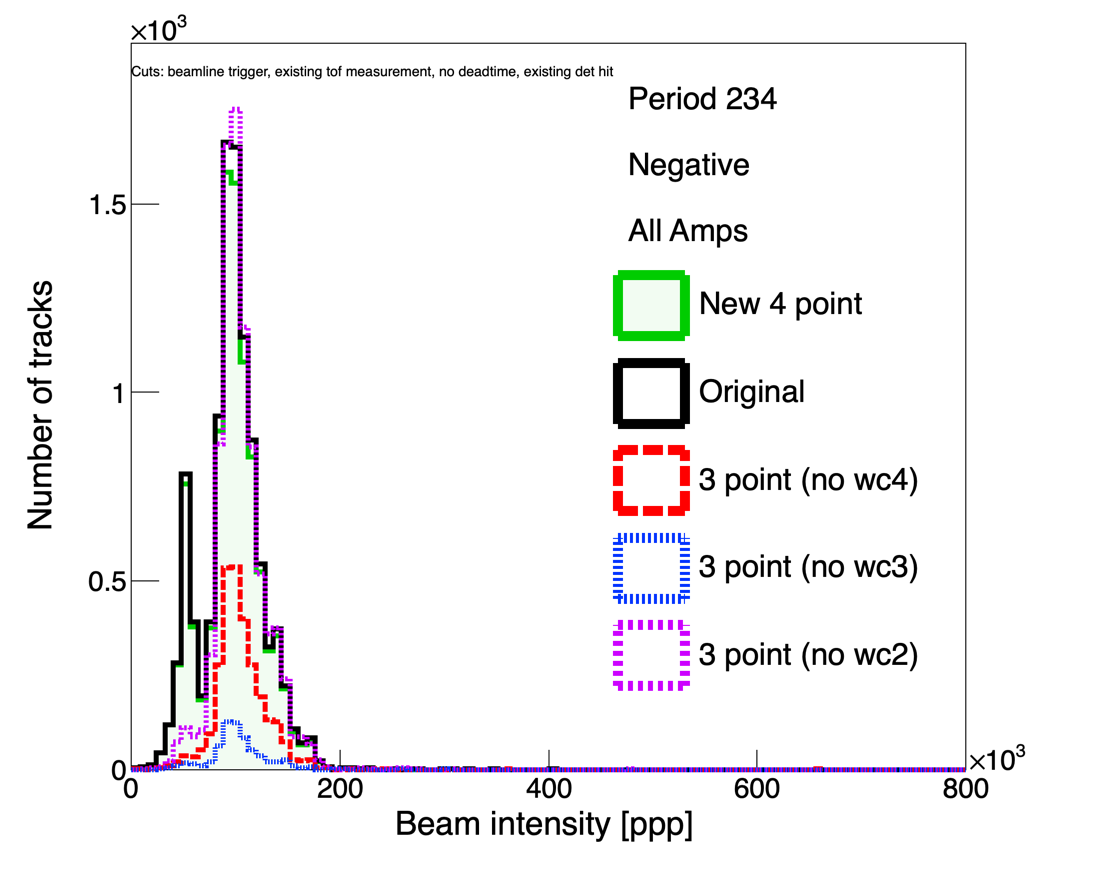
\includegraphics[scale=0.18]{NEW-figsingle_period234_intensity_level4_neg_stats_allAmps_nomomcut.png}
   \caption[short]{The beam intensity for top: no cuts, middle: trigger and tof cuts; bottom: + deadtime and detector hit cuts. Left is positive polarity, right is negative polarity.}
   \label{fig_intensity}
  \end{figure}
 
  \begin{figure}[h]
    \centering   
     	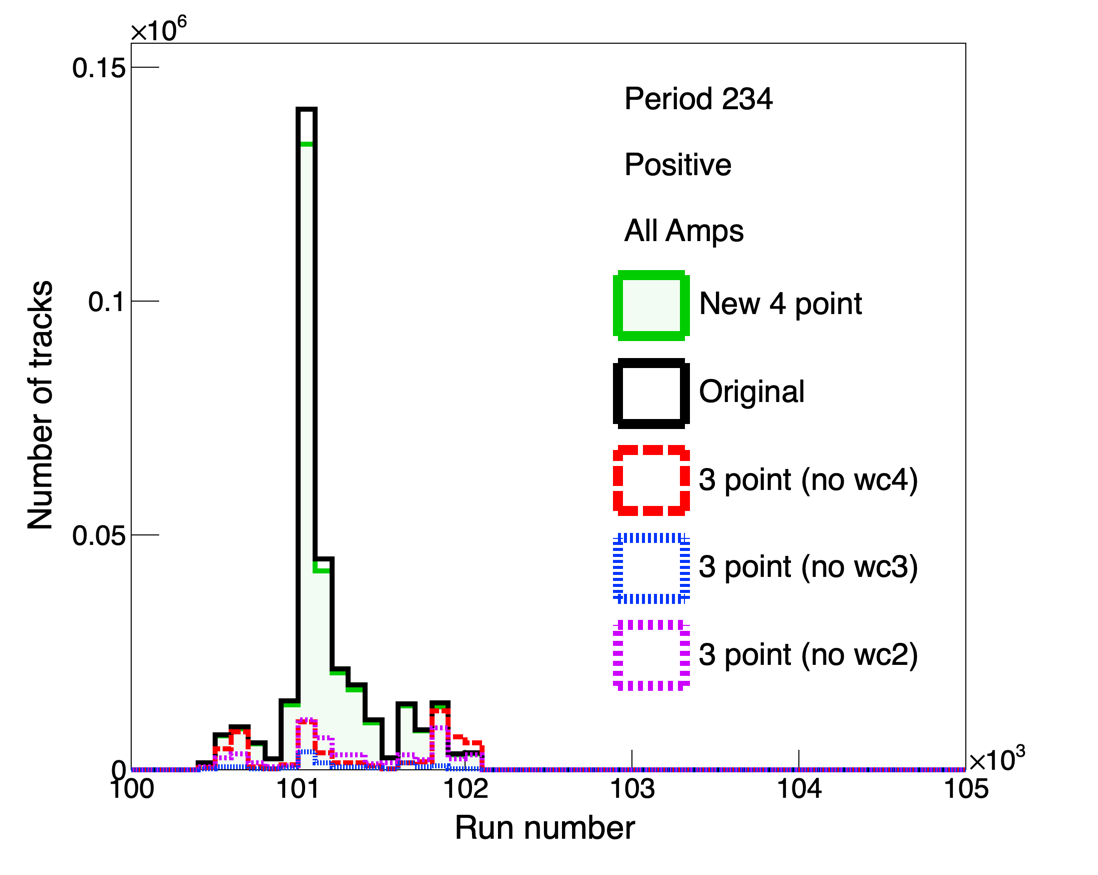
\includegraphics[scale=0.18]{NEW-figsingle_period234_run_level0_pos_stats_allAmps_nomomcut.png}
	 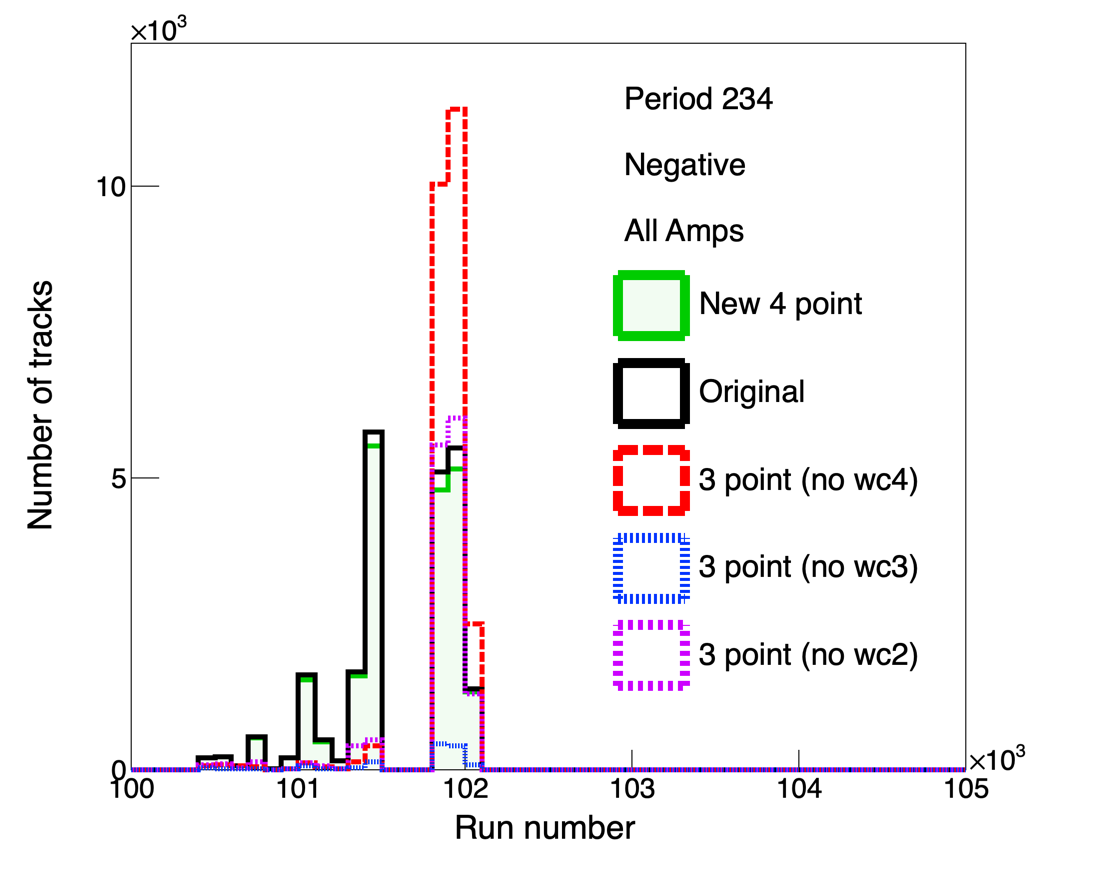
\includegraphics[scale=0.18]{NEW-figsingle_period234_run_level0_neg_stats_allAmps_nomomcut.png}
	 
   	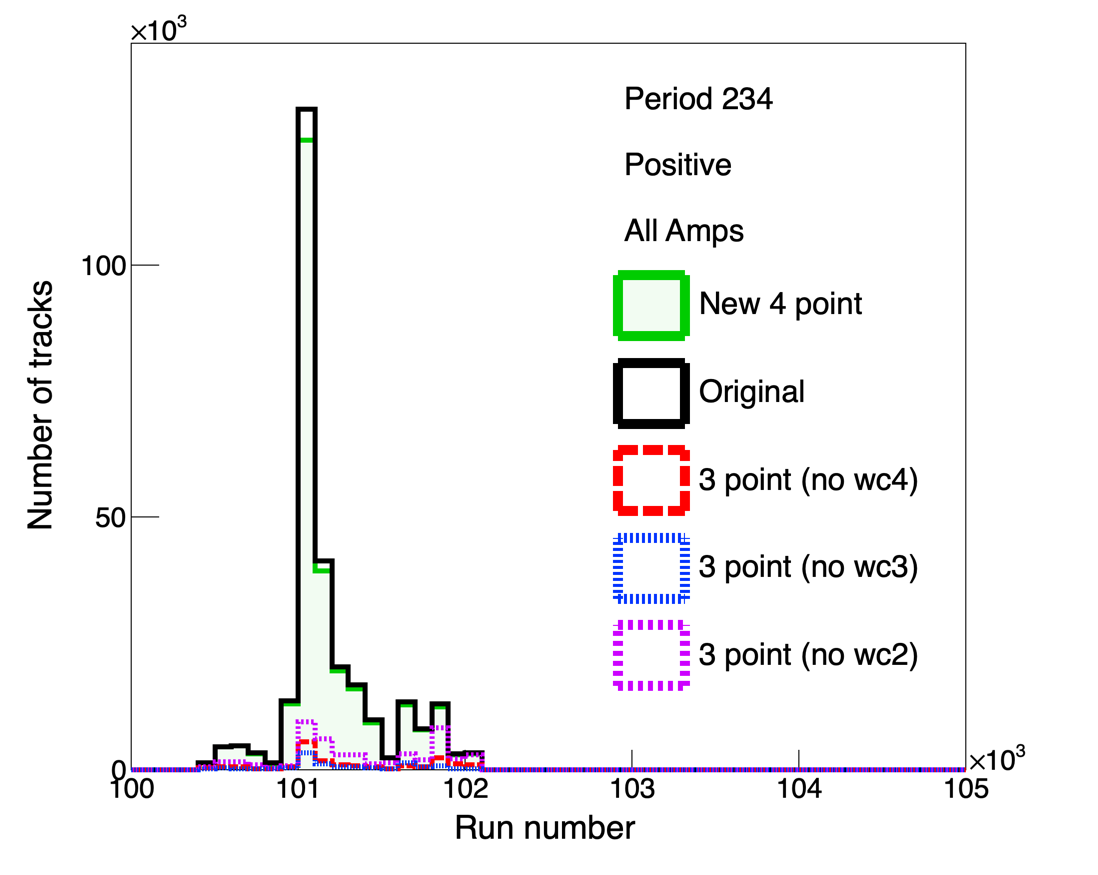
\includegraphics[scale=0.18]{NEW-figsingle_period234_run_level2_pos_stats_allAmps_nomomcut.png}
	 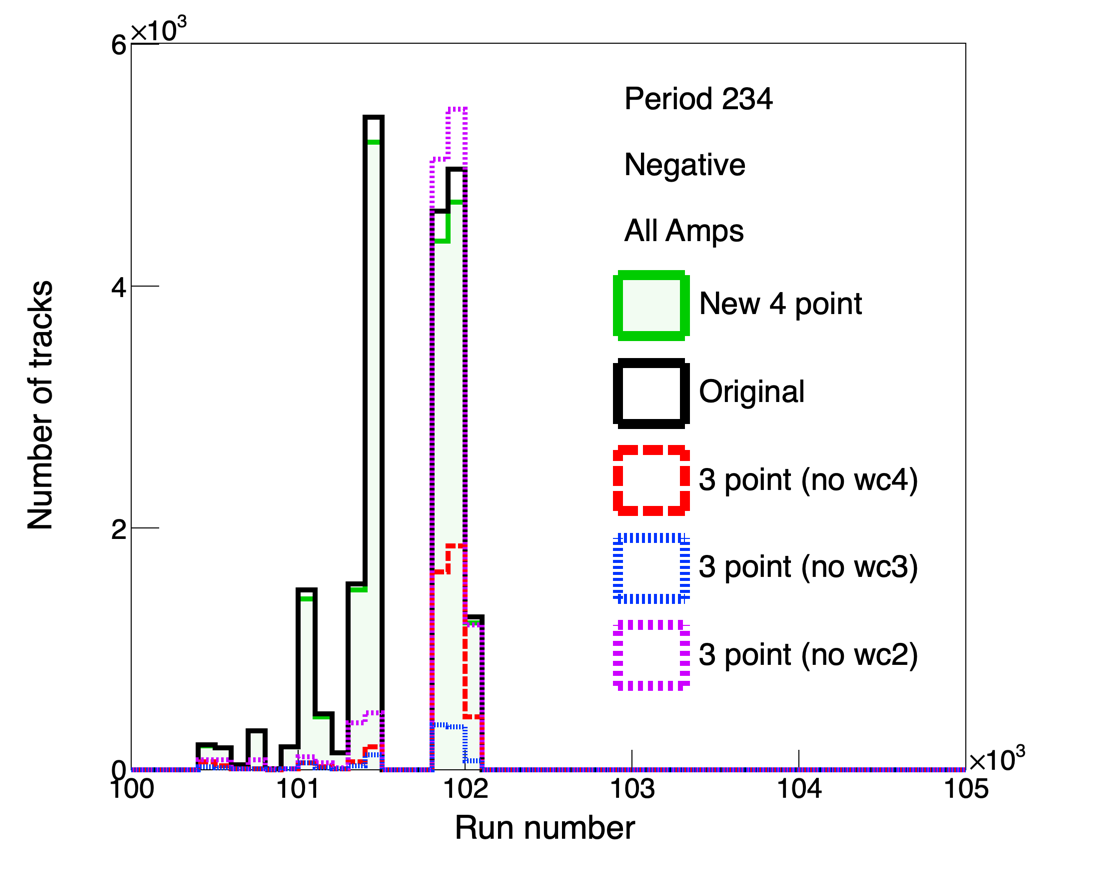
\includegraphics[scale=0.18]{NEW-figsingle_period234_run_level2_neg_stats_allAmps_nomomcut.png}
	 
 	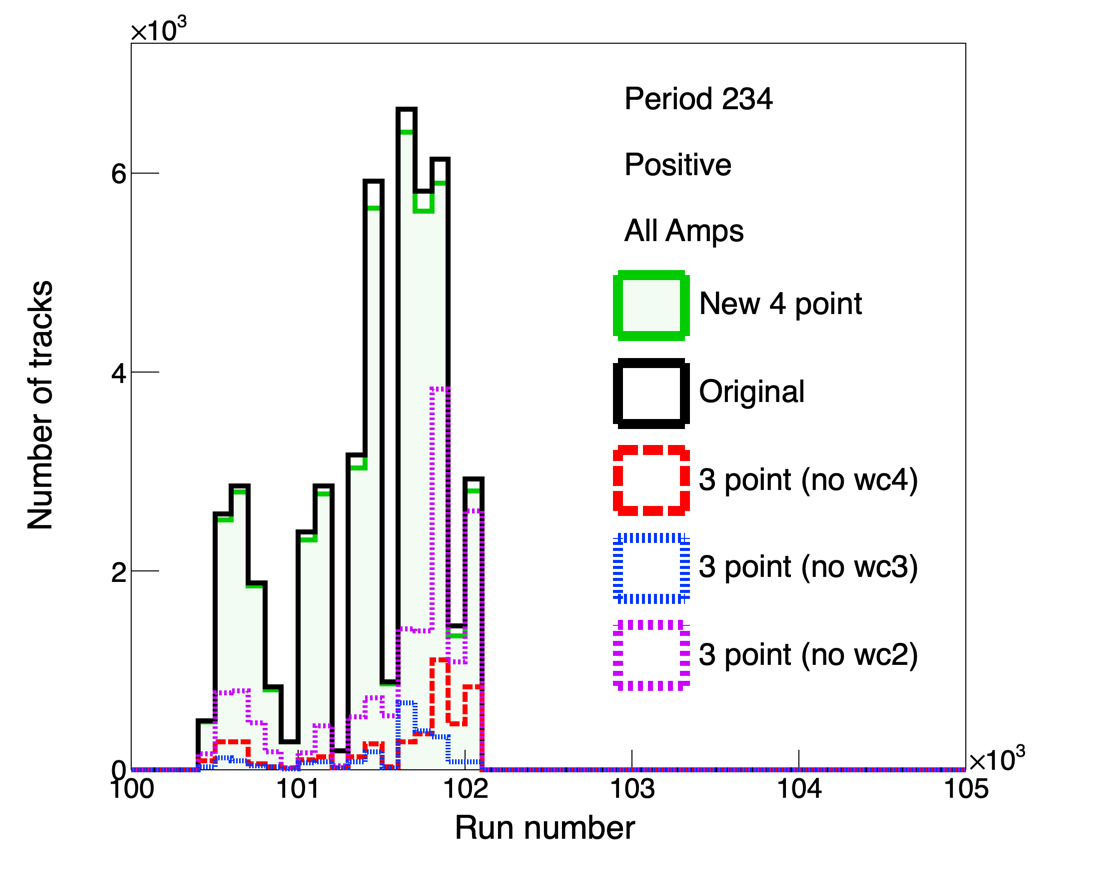
\includegraphics[scale=0.18]{NEW-figsingle_period234_run_level4_pos_stats_allAmps_nomomcut.png}
	 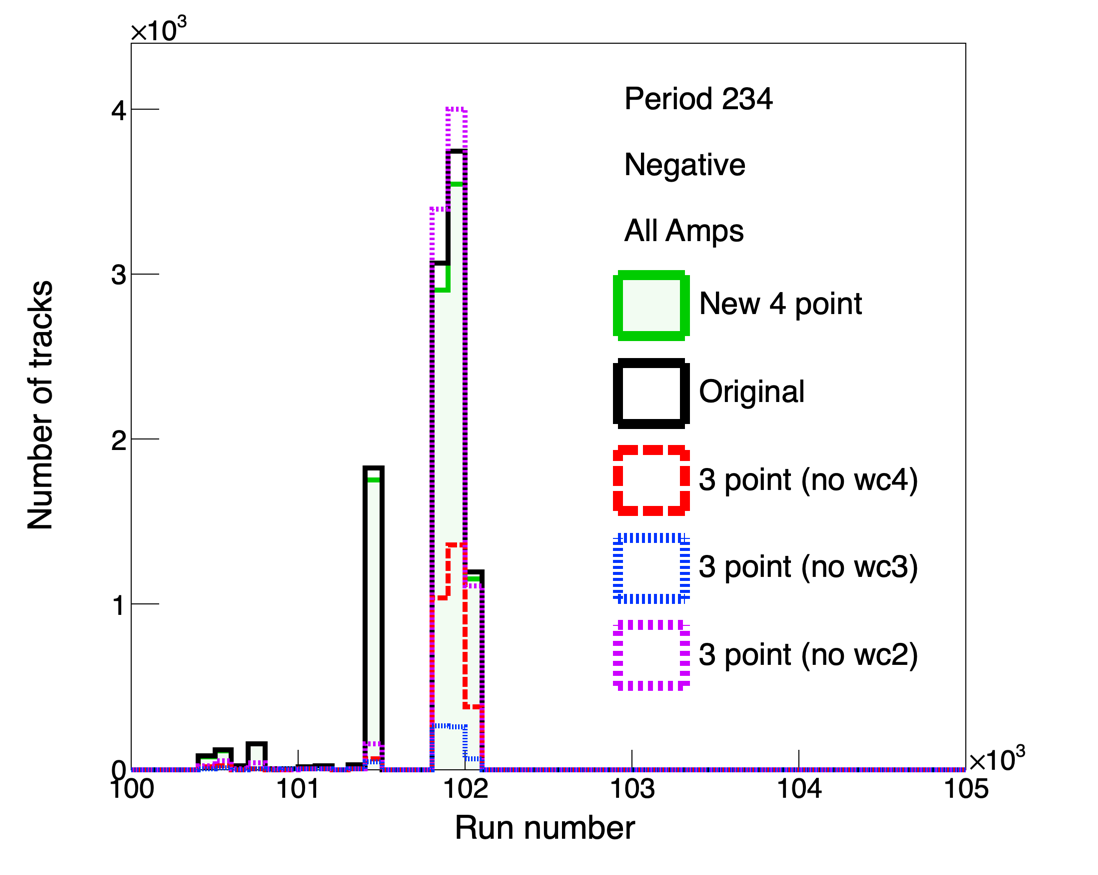
\includegraphics[scale=0.18]{NEW-figsingle_period234_run_level4_neg_stats_allAmps_nomomcut.png}
   \caption[short]{The run number for top: no cuts, middle: trigger and tof cuts; bottom: + deadtime and detector hit cuts. Left is positive polarity, right is negative polarity.}
   \label{fig_run}
  \end{figure}
  
  
  





\subsection{Comparing track properties}





 All of the original WCTrack properties have been kept to ensure back-compatibility. They are as follows:\\
 
 \begin{description}
 
 \item[WCTrack.Momentum()]{
 The reconstructed momentum corrected for magnetic field non-uniformity. Figure~\ref{fig_momentum} shows the momentum distributions for the 1000 Amp magnet current setting in the three periods for positive and negative polarity settings.
 I do not understand why the momentum distribution of the New 4 point tracks is skewed to higher momentum than the Original, which looks Gaussian. Want to add the un-corrected momentum distribution to see how much of the difference is coming from the geometry change. May actually be the only explanation.
 }
 
 
 
 \item[WCTrack.TransDistToMagAxis()]{
Transverse distance from WC track intercept to central axis of magnet. Figure~\ref{fig_magdist} shows the  distributions for the 1000 Amp magnet current setting in the three periods for positive and negative polarity settings.
  \begin{figure}[h]
    \centering   
     	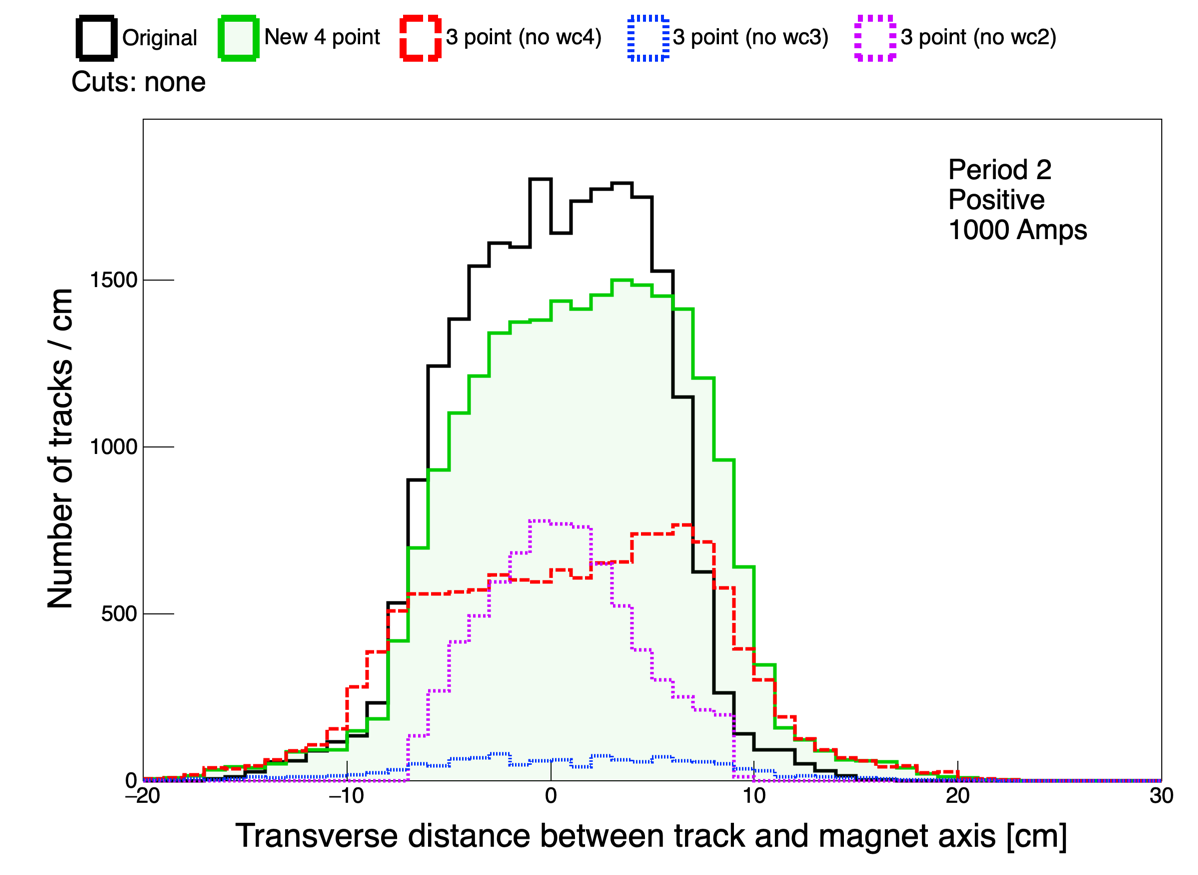
\includegraphics[scale=0.18]{NEW-figsingle_period2_magdist_level0_pos_stats_1000Amps.png}
	 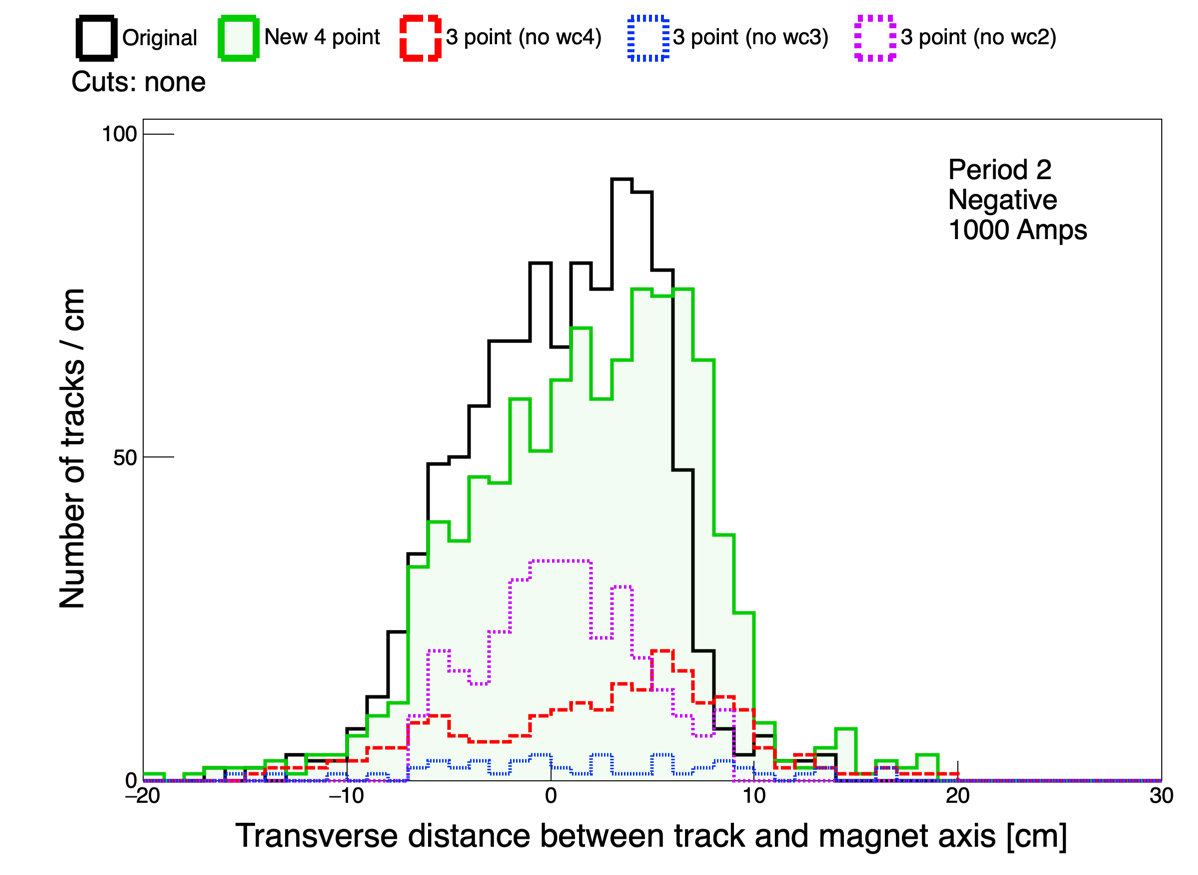
\includegraphics[scale=0.18]{NEW-figsingle_period2_magdist_level0_neg_stats_1000Amps.png}
	 
   	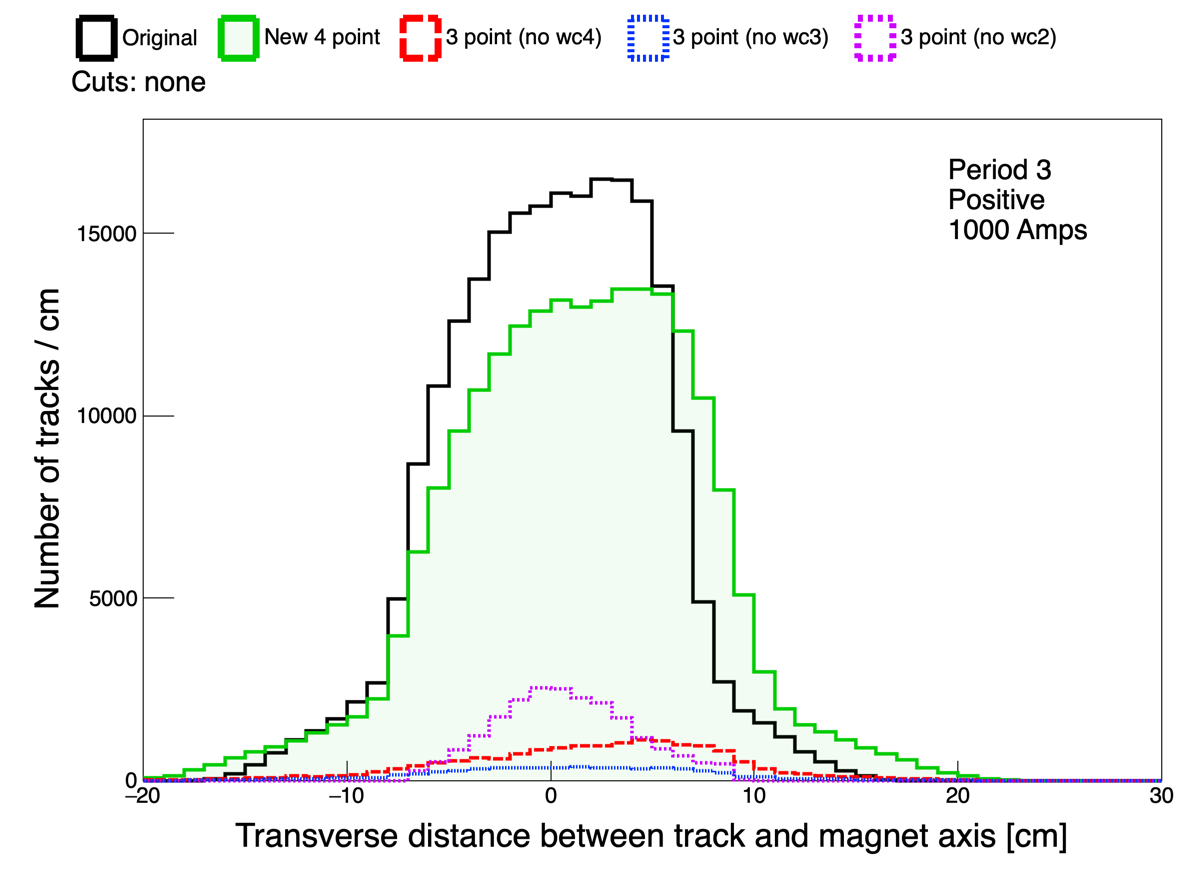
\includegraphics[scale=0.18]{NEW-figsingle_period3_magdist_level0_pos_stats_1000Amps.png}
	 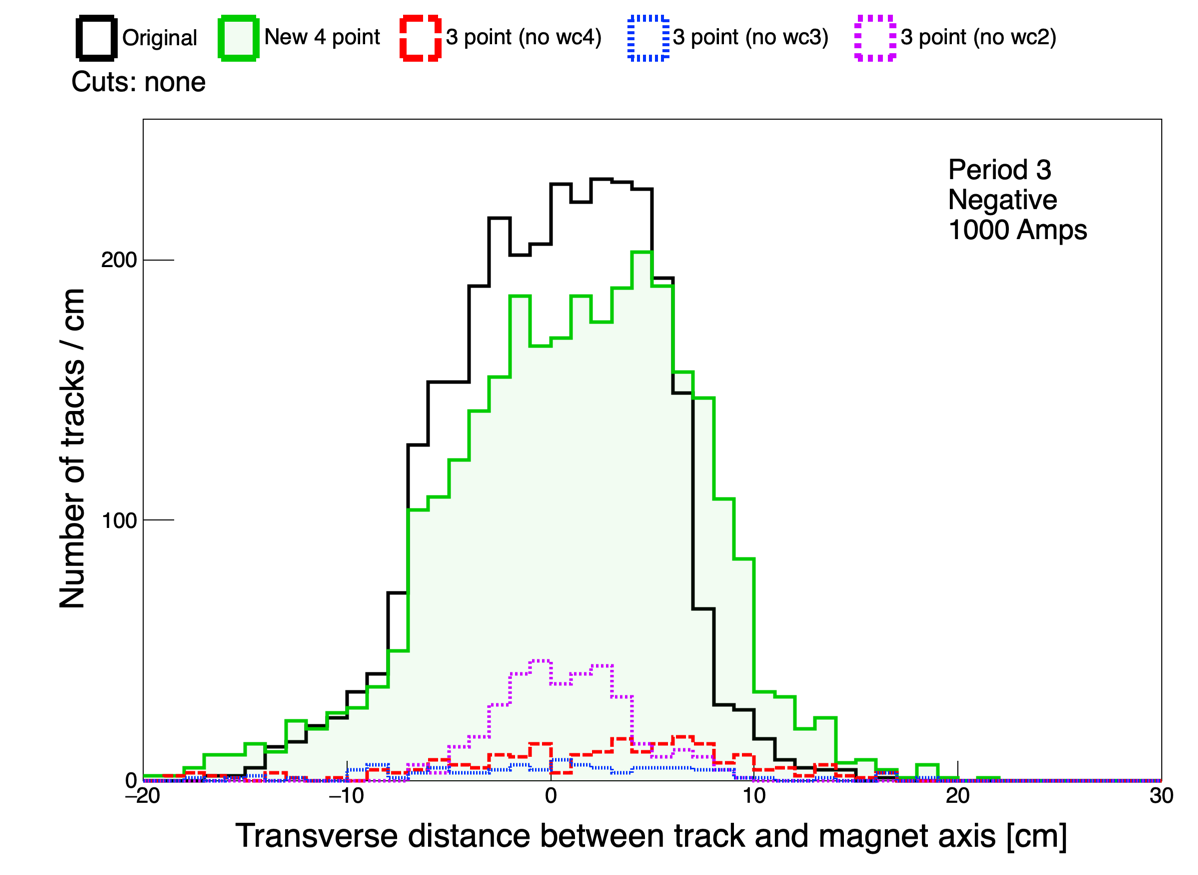
\includegraphics[scale=0.18]{NEW-figsingle_period3_magdist_level0_neg_stats_1000Amps.png}
	 
 	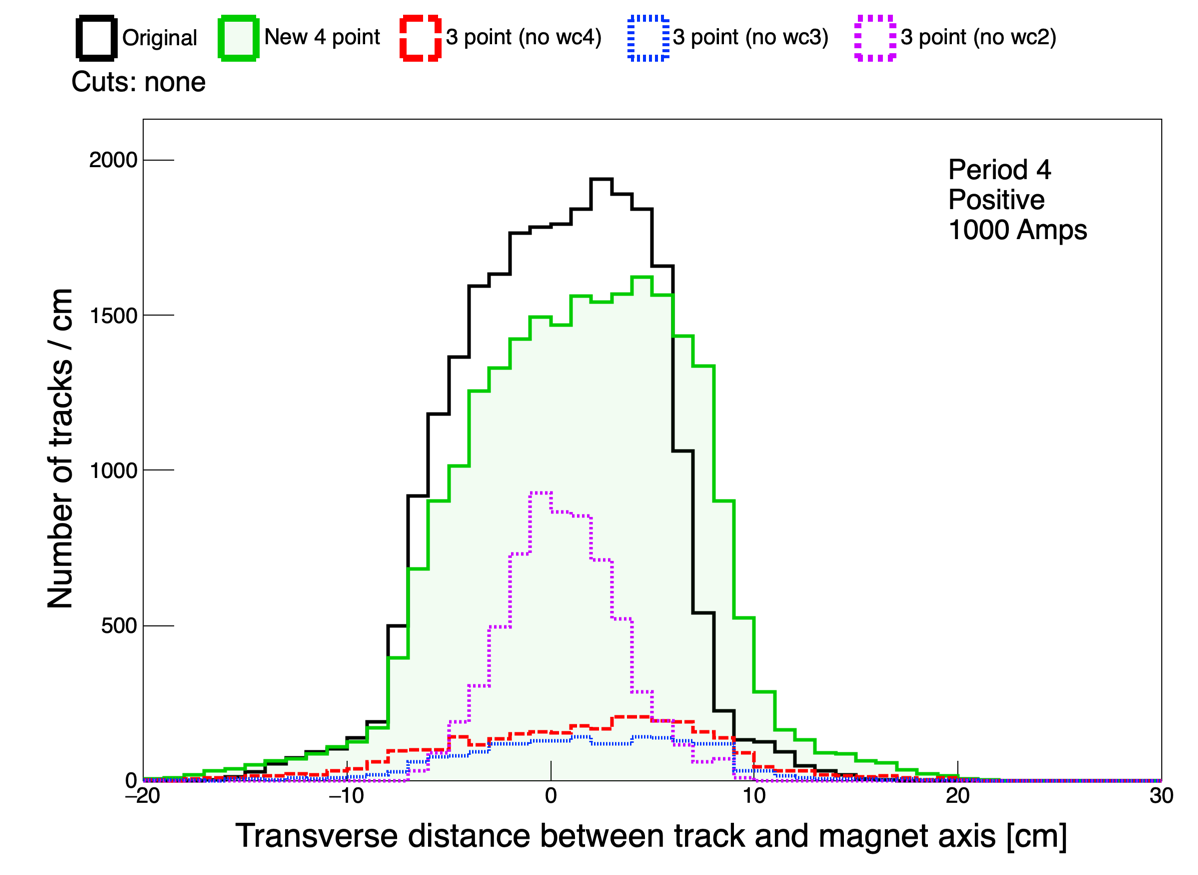
\includegraphics[scale=0.18]{NEW-figsingle_period4_magdist_level0_pos_stats_1000Amps.png}
	 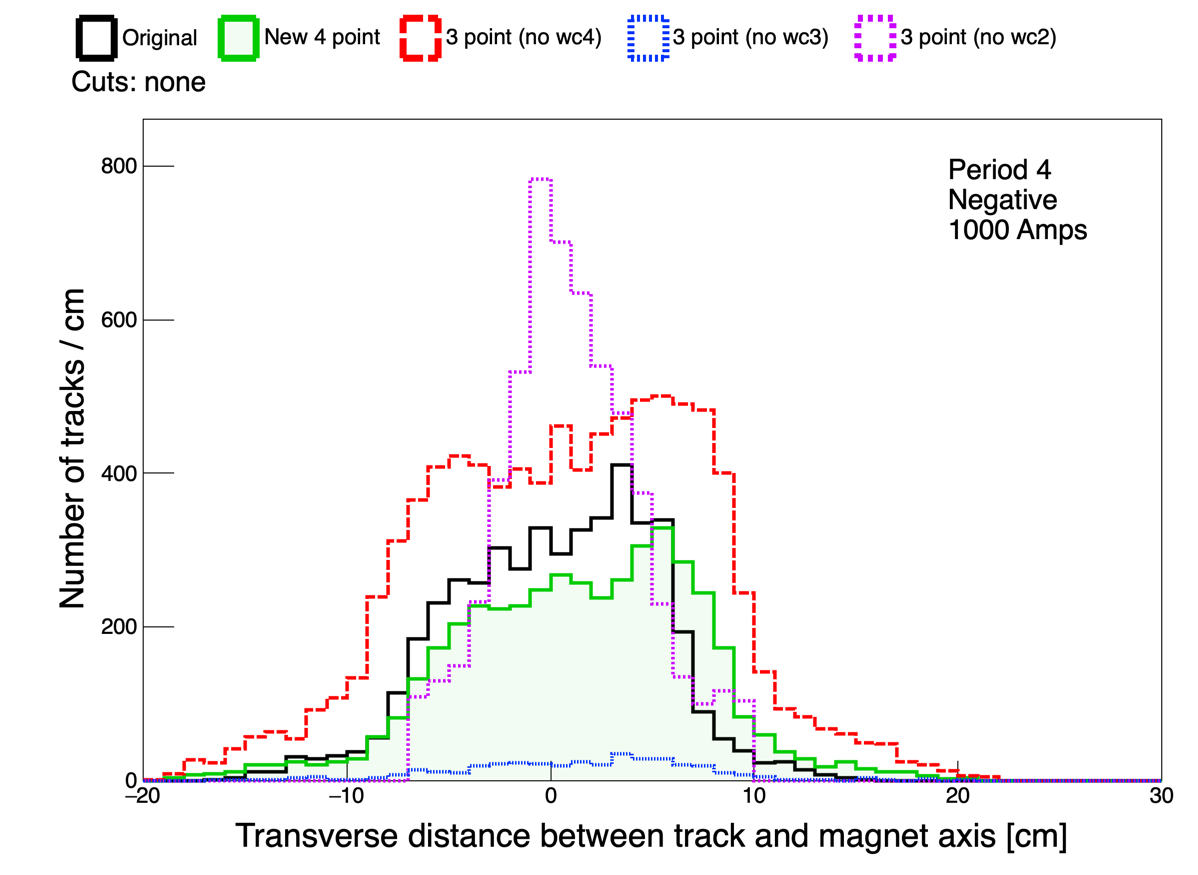
\includegraphics[scale=0.18]{NEW-figsingle_period4_magdist_level0_neg_stats_1000Amps.png}
   \caption[short]{The WCTrack magnet distance with magnet current 1000 Amps. Left: positive polarity, Right: negative polarity, Top: period 3, Bottom: period 4. No cuts applied.}
   \label{fig_magdist}
  \end{figure}
 
}


 
 % Figures \ref{fig:p12_neg} (for negative polarity) and  \ref{fig:p12_pos} (for positive polarity) show a comparison between the original and the new implementation of WCTrackAlg, including 3-point tracks broken down by which of the wirechamber hits is missing. 
 
 
 
 \begin{figure}
   \centering   
 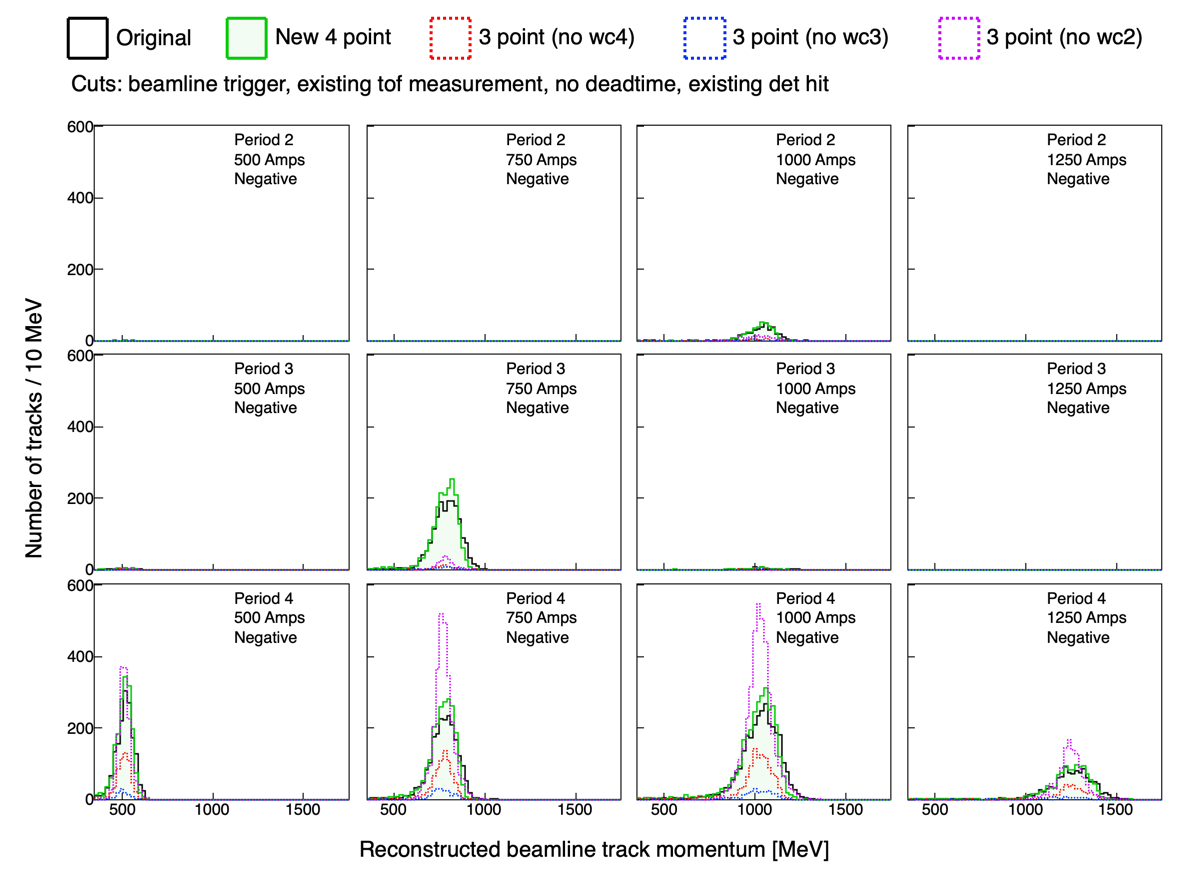
\includegraphics[scale=0.35]{fig_p_level4_neg_stats.png}
 \caption[short]{The WCTrack momentum for negative polarity broken down by row: period and column: magnet current setting. There is a common y-axis scale for all plots.}
 \label{fig:p12_neg}
  \end{figure}
 
 
  \begin{figure}
    \centering   
 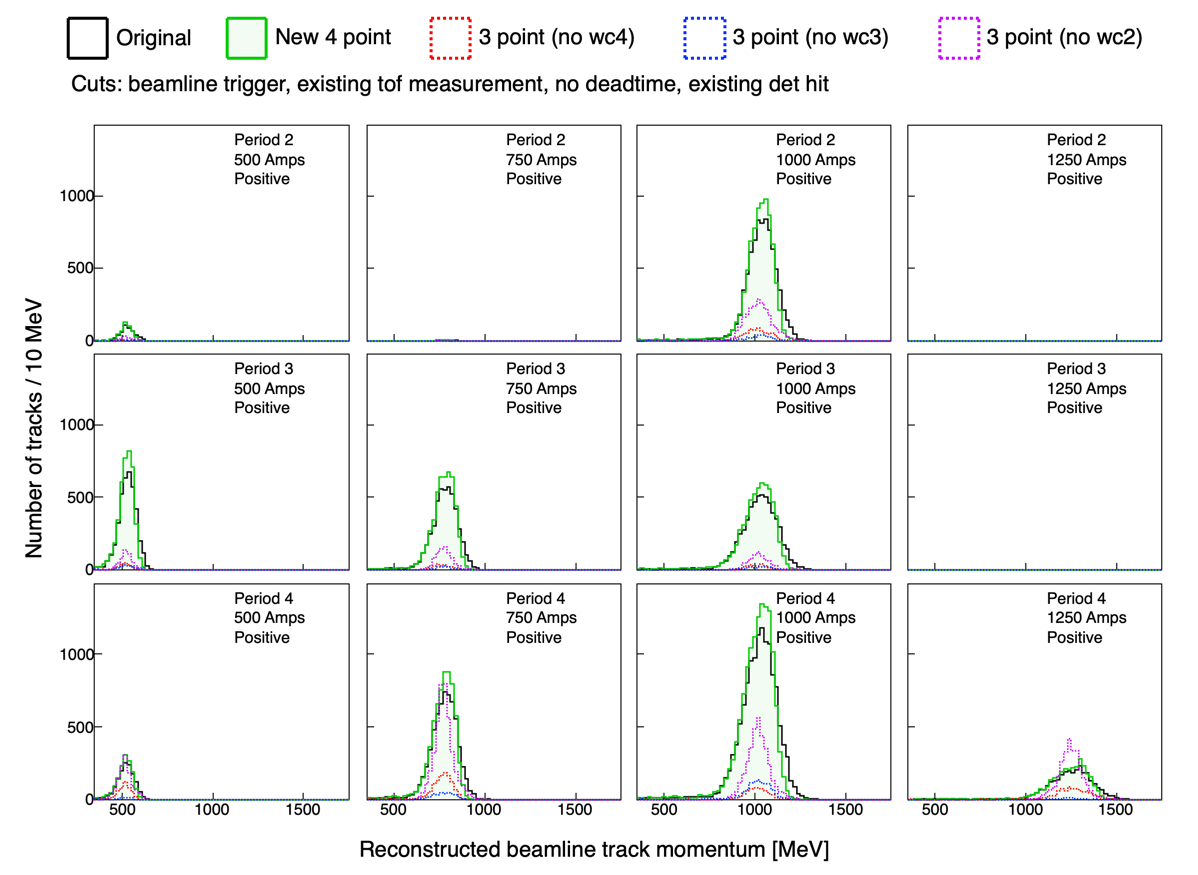
\includegraphics[scale=0.35]{fig_p_level4_pos_stats.png}
 \caption[short]{The WCTrack momentum for positive polarity broken down by row: period and column: magnet current setting. There is a common y-axis scale for all plots.}
 \label{fig:p12_pos}
  \end{figure}
  
  
  
  \item[WCTrack.YKink()] {  Angle difference dy/dz  between upstream and downstream tracks. Figure~\ref{fig_ykink} shows the  distributions for the 1000 Amp magnet current setting in the three periods for positive and negative polarity settings.
    \begin{figure}[h]
      \centering   
       	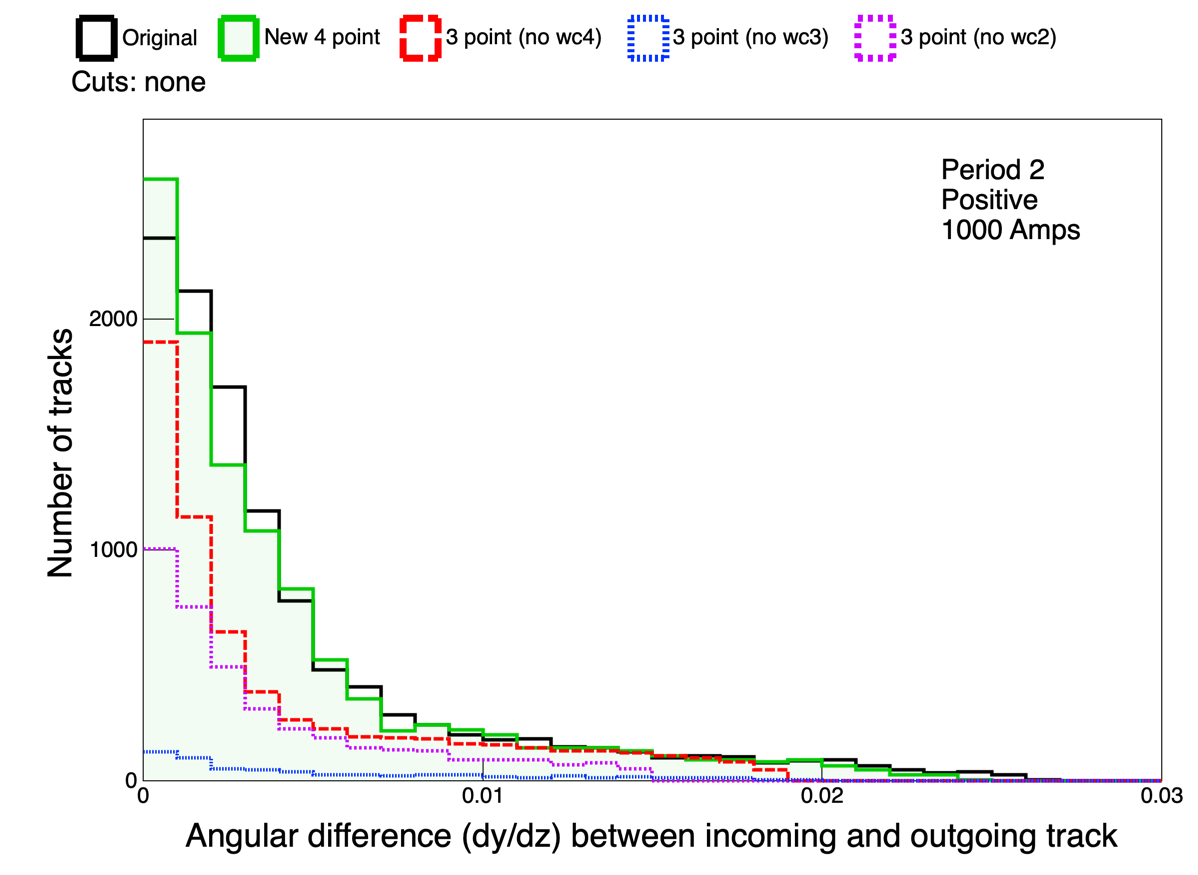
\includegraphics[scale=0.18]{NEW-figsingle_period2_ykink_level0_pos_stats_1000Amps.png}
	 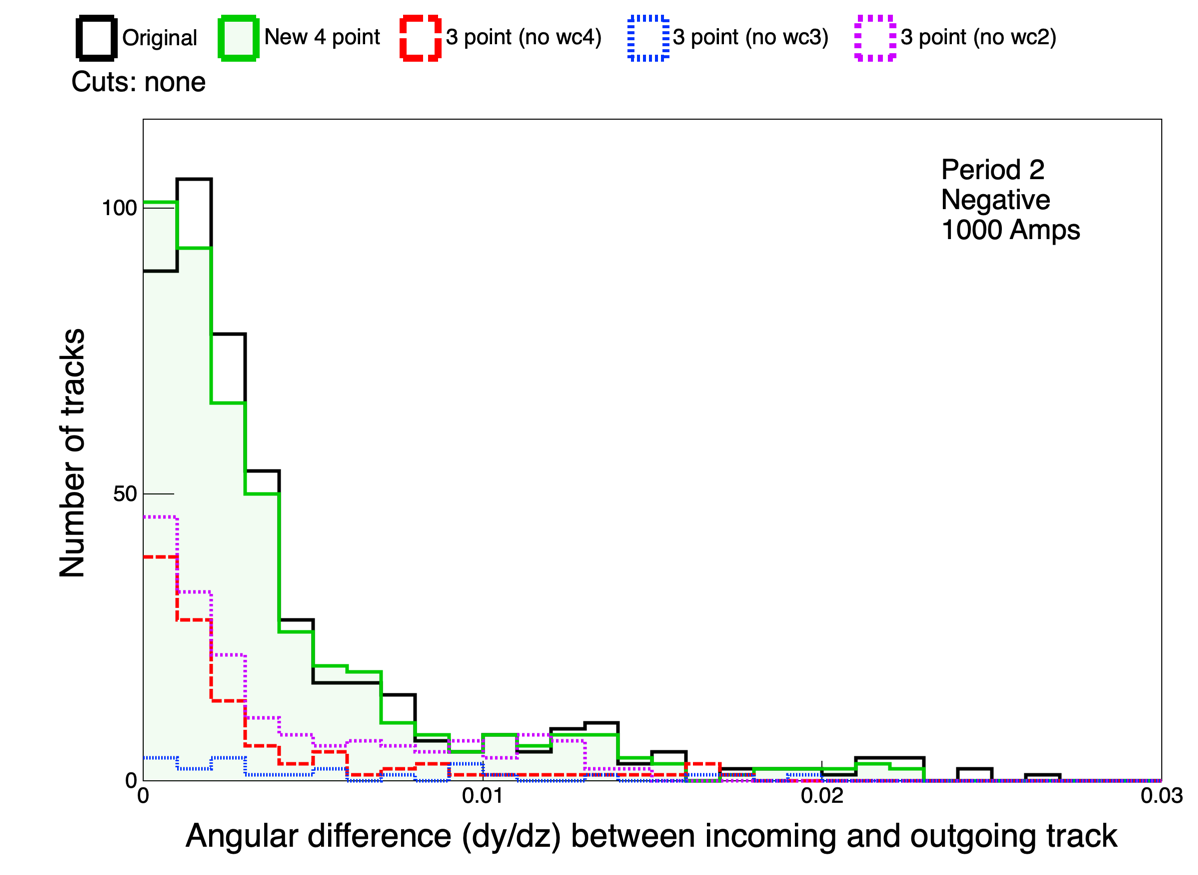
\includegraphics[scale=0.18]{NEW-figsingle_period2_ykink_level0_neg_stats_1000Amps.png}
	 
   	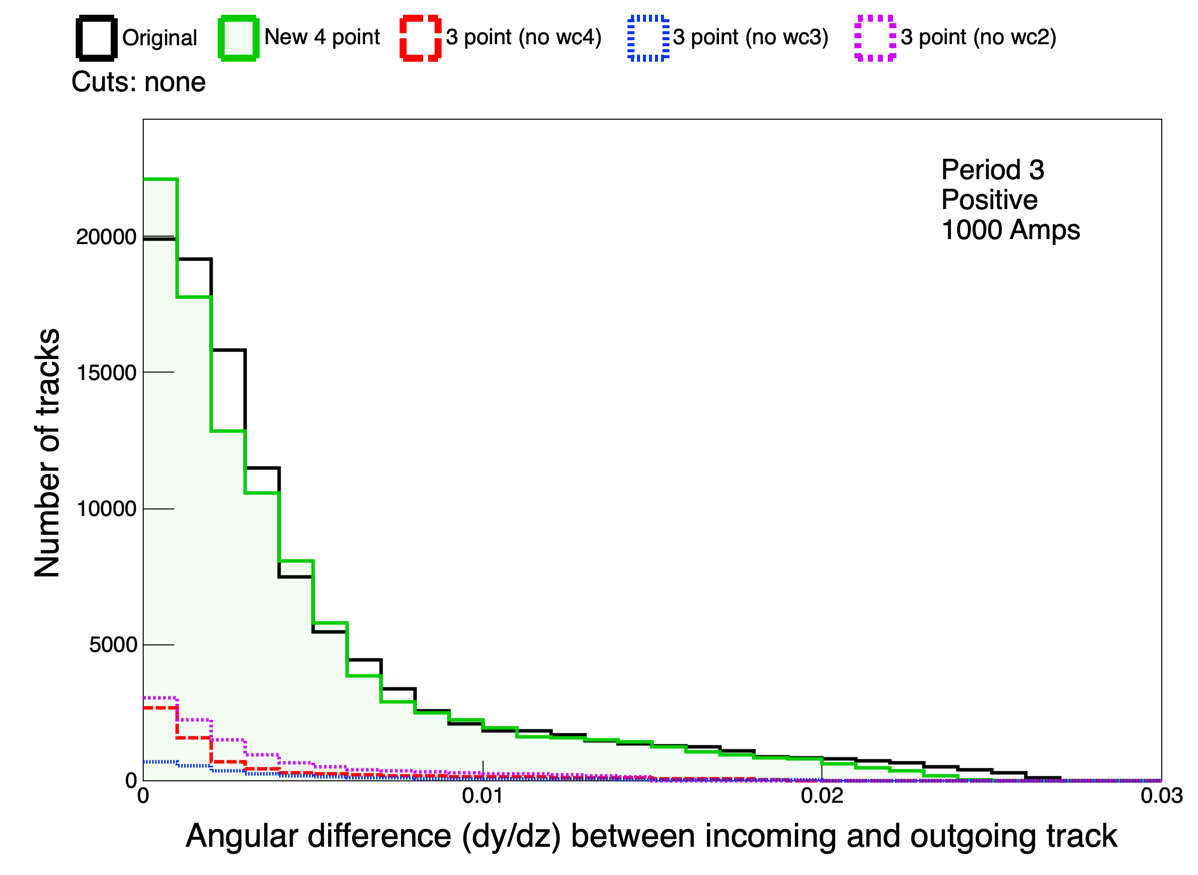
\includegraphics[scale=0.18]{NEW-figsingle_period3_ykink_level0_pos_stats_1000Amps.png}
	 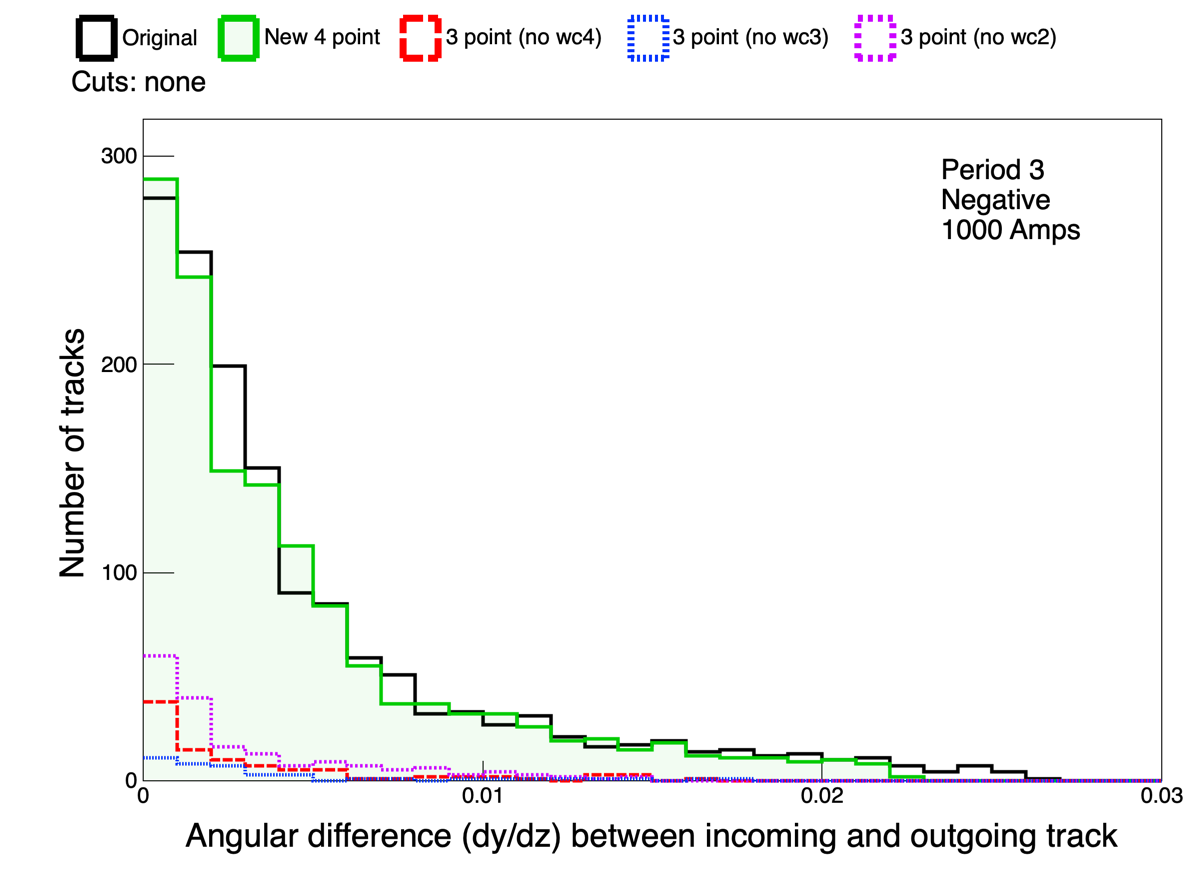
\includegraphics[scale=0.18]{NEW-figsingle_period3_ykink_level0_neg_stats_1000Amps.png}
	 
 	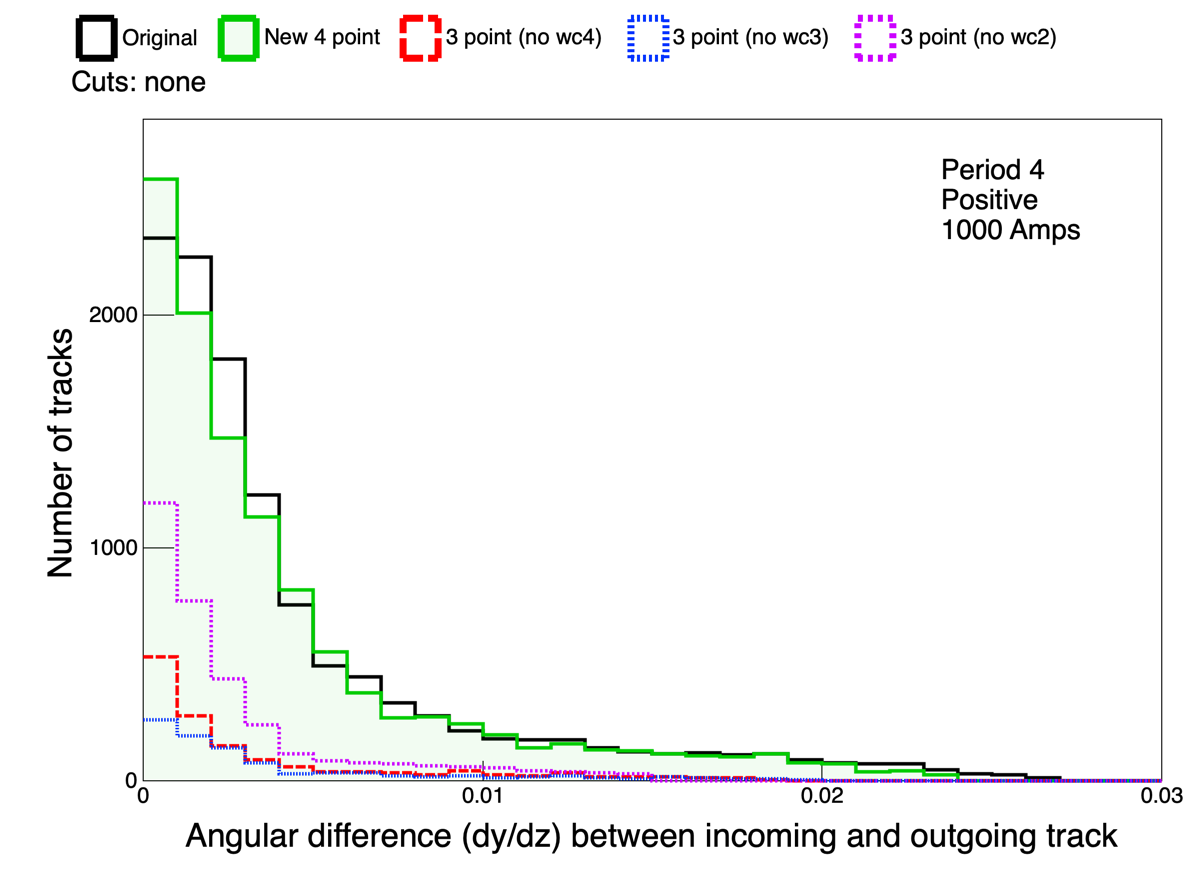
\includegraphics[scale=0.18]{NEW-figsingle_period4_ykink_level0_pos_stats_1000Amps.png}
	 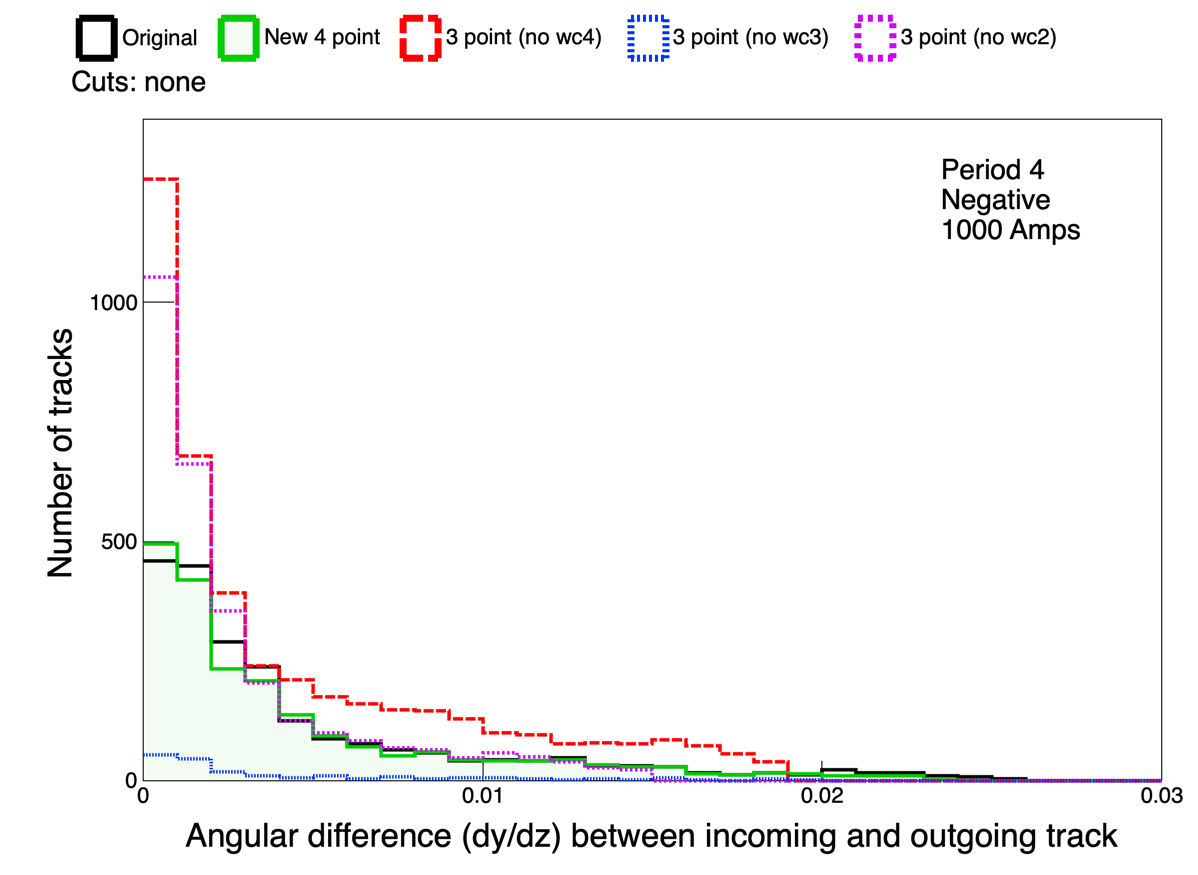
\includegraphics[scale=0.18]{NEW-figsingle_period4_ykink_level0_neg_stats_1000Amps.png}
   \caption[short]{The WCTrack ykink with magnet current 1000 Amps. Left: positive polarity, Right: negative polarity, Top: period 3, Bottom: period 4. No cuts applied.}
   \label{fig_ykink}
  \end{figure}
  }
  
 \item[WCTrack.Residual()] {   
   Returns the average residual, indicating the goodness of fit to a linear regression for the points used in the track. Figure~\ref{fig_residual} shows the  distributions for the 1000 Amp magnet current setting in the three periods for positive and negative polarity settings. Note that the definition of the residual is different in the case of the original WCTrack from the new 4 and 3 point tracks, as described in Section~\ref{sec_residual}.
         \begin{figure}[h]
           \centering   
            	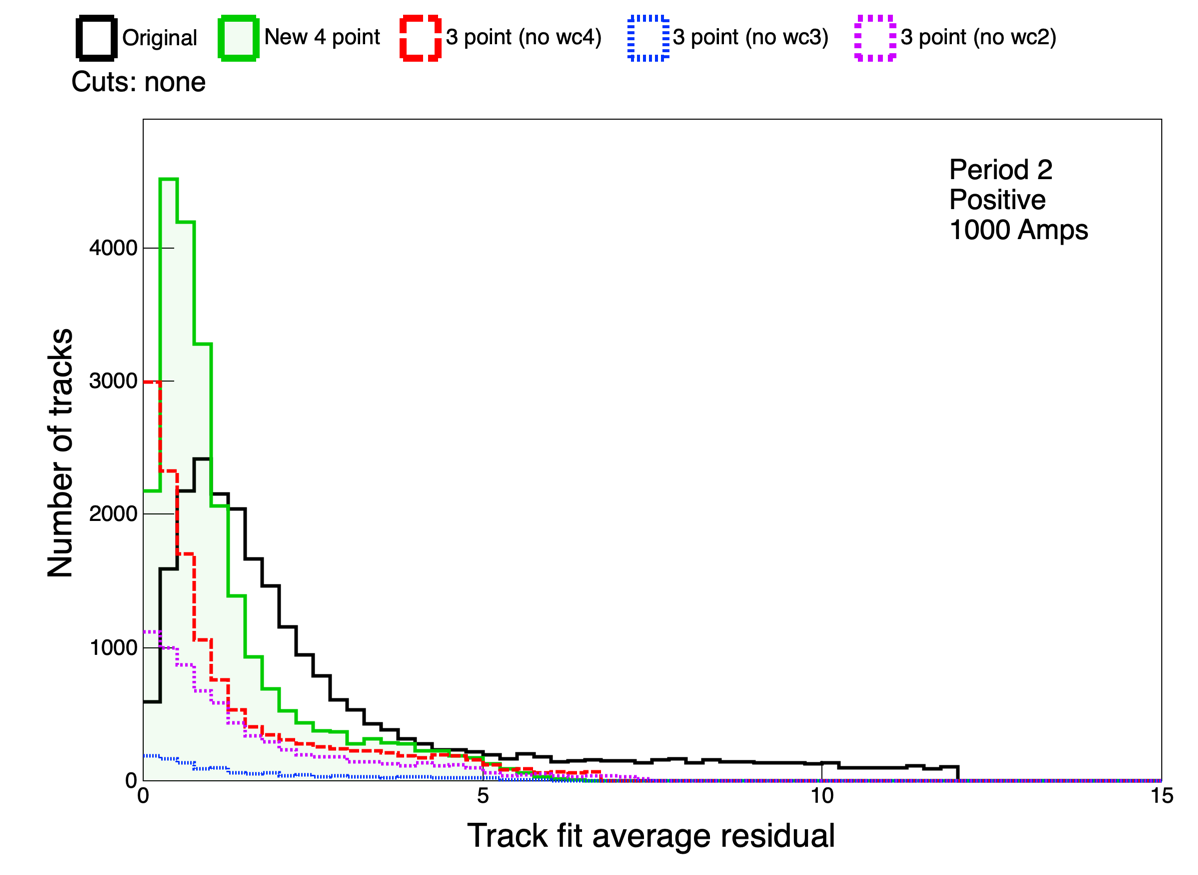
\includegraphics[scale=0.18]{NEW-figsingle_period2_residual_level0_pos_stats_1000Amps.png}
	 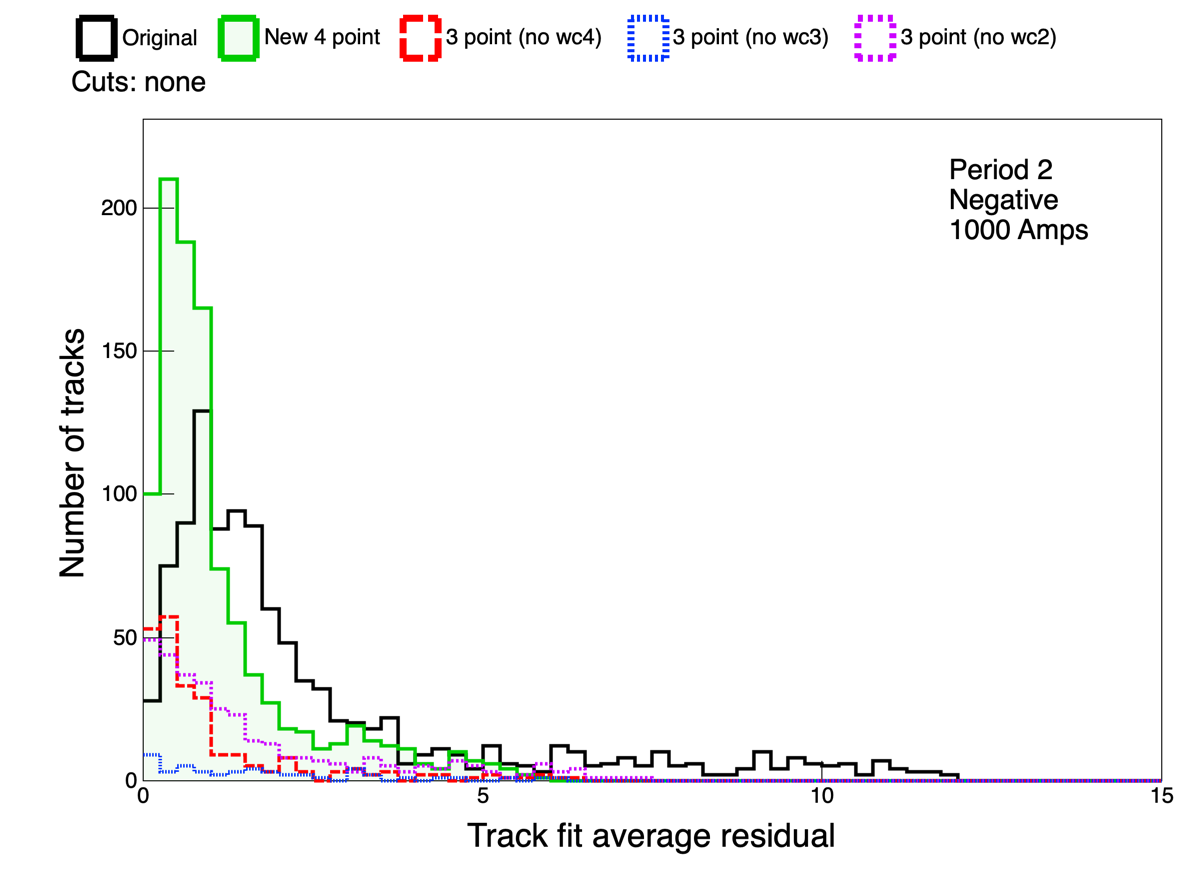
\includegraphics[scale=0.18]{NEW-figsingle_period2_residual_level0_neg_stats_1000Amps.png}
	 
   	\includegraphics[scale=0.18]{NEW-figsingle_period3_residual_level0_pos_stats_1000Amps.png}
	 \includegraphics[scale=0.18]{NEW-figsingle_period3_residual_level0_neg_stats_1000Amps.png}
	 
 	\includegraphics[scale=0.18]{NEW-figsingle_period4_residual_level0_pos_stats_1000Amps.png}
	 \includegraphics[scale=0.18]{NEW-figsingle_period4_residual_level0_neg_stats_1000Amps.png}
   \caption[short]{The WCTrack residual with magnet current 1000 Amps. Left: positive polarity, Right: negative polarity, Top: period 3, Bottom: period 4. No cuts applied. .}
   \label{fig_residual}
  \end{figure}
 }
   
\item[WCTrack.XYFace]{
  X and Y position of the track on the upstream face of the detector. Figure~\ref{fig_x} and  \ref{fig_y} show the distributions for the 1000 Amp magnet current setting in the three periods for positive and negative polarity settings.
      \begin{figure}[h]
        \centering   
         	\includegraphics[scale=0.18]{NEW-figsingle_period2_x_level0_pos_stats_1000Amps.png}
	 \includegraphics[scale=0.18]{NEW-figsingle_period2_x_level0_neg_stats_1000Amps.png}
	 
   	\includegraphics[scale=0.18]{NEW-figsingle_period3_x_level0_pos_stats_1000Amps.png}
	 \includegraphics[scale=0.18]{NEW-figsingle_period3_x_level0_neg_stats_1000Amps.png}
	 
 	\includegraphics[scale=0.18]{NEW-figsingle_period4_x_level0_pos_stats_1000Amps.png}
	 \includegraphics[scale=0.18]{NEW-figsingle_period4_x_level0_neg_stats_1000Amps.png}
   \caption[short]{The WCTrack x with magnet current 1000 Amps. Left: positive polarity, Right: negative polarity, Top: period 3, Bottom: period 4. No cuts applied.}
   \label{fig_x}
  \end{figure}
  
      \begin{figure}[h]
        \centering   
         	\includegraphics[scale=0.18]{NEW-figsingle_period2_y_level0_pos_stats_1000Amps.png}
	 \includegraphics[scale=0.18]{NEW-figsingle_period2_y_level0_neg_stats_1000Amps.png}
	 
   	\includegraphics[scale=0.18]{NEW-figsingle_period3_y_level0_pos_stats_1000Amps.png}
	 \includegraphics[scale=0.18]{NEW-figsingle_period3_y_level0_neg_stats_1000Amps.png}
	 
 	\includegraphics[scale=0.18]{NEW-figsingle_period4_y_level0_pos_stats_1000Amps.png}
	 \includegraphics[scale=0.18]{NEW-figsingle_period4_y_level0_neg_stats_1000Amps.png}
   \caption[short]{The WCTrack y with magnet current 1000 Amps. Left: positive polarity, Right: negative polarity, Top: period 3, Bottom: period 4. No cuts applied.}
   \label{fig_y}
  \end{figure}
  
  
 }


\item[WCTrack.DeltaDist()]{
Distance between upstream and downstream track ends. The x, y, z intercepts of both the upstream an downstream portions of each track are calculated, and the difference between upstream and downstream is the DeltaDist. Figure~\ref{fig_ddx}  shows a notable difference in the original tracking algorithm, which is centred around 150cm,  and the new implementation which is centred around zero. The track is expected to be diverted in the x-direction due to magnetic field, so I do not understand why the new implementation gives a distribution around zero. \textcolor{red}{check the implementation of DeltaDist}. The y-dsstribution in Figure~\ref{fig_ddy} also shows a difference, with the delta dy distribution being more sharlpy peaked in the original WCTrack implementation.  In this case though both the original and new implementations have a delta dy peaking about zero, which is what I would expect. finally the delta dx distribution shown in Figure~\ref{fig_ddz} echoes the delta dx distribution differences, but in this case the original delta dz distribution is shifted by just over 20cm. I don't understand this. 

 \begin{figure}[h]	 
   \centering   
    	\includegraphics[scale=0.18]{NEW-figsingle_period2_ddx_level0_pos_stats_1000Amps.png}
	 \includegraphics[scale=0.18]{NEW-figsingle_period2_ddx_level0_neg_stats_1000Amps.png}
	 
   	\includegraphics[scale=0.18]{NEW-figsingle_period3_ddx_level0_pos_stats_1000Amps.png}
	 \includegraphics[scale=0.18]{NEW-figsingle_period3_ddx_level0_neg_stats_1000Amps.png}
	 
 	\includegraphics[scale=0.18]{NEW-figsingle_period4_ddx_level0_pos_stats_1000Amps.png}
	 \includegraphics[scale=0.18]{NEW-figsingle_period4_ddx_level0_neg_stats_1000Amps.png}
   \caption[short]{The WCTrack delta dx with magnet current 1000 Amps. Left: positive polarity, Right: negative polarity, Top: period 3, Bottom: period 4. No cuts applied.}
   \label{fig_ddx}
  \end{figure}
  
  
   \begin{figure}[h]	 
     \centering   
   
      	\includegraphics[scale=0.18]{NEW-figsingle_period2_ddy_level0_pos_stats_1000Amps.png}
	 \includegraphics[scale=0.18]{NEW-figsingle_period2_ddy_level0_neg_stats_1000Amps.png}
	 
   	\includegraphics[scale=0.18]{NEW-figsingle_period3_ddy_level0_pos_stats_1000Amps.png}
	 \includegraphics[scale=0.18]{NEW-figsingle_period3_ddy_level0_neg_stats_1000Amps.png}
	 
 	\includegraphics[scale=0.18]{NEW-figsingle_period4_ddy_level0_pos_stats_1000Amps.png}
	 \includegraphics[scale=0.18]{NEW-figsingle_period4_ddy_level0_neg_stats_1000Amps.png}
   \caption[short]{The WCTrack delta dy with magnet current 1000 Amps. Left: positive polarity, Right: negative polarity, Top: period 3, Bottom: period 4. No cuts applied.}
   \label{fig_ddy}
  \end{figure}
  
     \begin{figure}[h]	 
       \centering   
     
        	\includegraphics[scale=0.18]{NEW-figsingle_period2_ddz_level0_pos_stats_1000Amps.png}
	 \includegraphics[scale=0.18]{NEW-figsingle_period2_ddz_level0_neg_stats_1000Amps.png}
	 
   	\includegraphics[scale=0.18]{NEW-figsingle_period3_ddz_level0_pos_stats_1000Amps.png}
	 \includegraphics[scale=0.18]{NEW-figsingle_period3_ddz_level0_neg_stats_1000Amps.png}
	 
 	\includegraphics[scale=0.18]{NEW-figsingle_period4_ddz_level0_pos_stats_1000Amps.png}
	 \includegraphics[scale=0.18]{NEW-figsingle_period4_ddz_level0_neg_stats_1000Amps.png}
   \caption[short]{The WCTrack delta dz with magnet current 1000 Amps. Left: positive polarity, Right: negative polarity, Top: period 3, Bottom: period 4. No cuts applied.}
   \label{fig_ddz}
  \end{figure}

}
\item[WCTrack.MagnetEntryPoint()]{
X,Y,Z intersect of upstream WC track with front face of magnet  X, Y, Z.

     \begin{figure}[h]	  
       \centering       
        	\includegraphics[scale=0.18]{NEW-figsingle_period2_mex_level0_pos_stats_1000Amps.png}
	 \includegraphics[scale=0.18]{NEW-figsingle_period2_mex_level0_neg_stats_1000Amps.png}
	 
   	\includegraphics[scale=0.18]{NEW-figsingle_period3_mex_level0_pos_stats_1000Amps.png}
	 \includegraphics[scale=0.18]{NEW-figsingle_period3_mex_level0_neg_stats_1000Amps.png}
	 
 	\includegraphics[scale=0.18]{NEW-figsingle_period4_mex_level0_pos_stats_1000Amps.png}
	 \includegraphics[scale=0.18]{NEW-figsingle_period4_mex_level0_neg_stats_1000Amps.png}
   \caption[short]{The WCTrack magnet entry x with magnet current 1000 Amps. Left: positive polarity, Right: negative polarity, Top: period 3, Bottom: period 4. No cuts applied.}
   \label{fig_mex}
  \end{figure}
  
       \begin{figure}[h]	
         \centering      
        	\includegraphics[scale=0.18]{NEW-figsingle_period2_mey_level0_pos_stats_1000Amps.png}
	 \includegraphics[scale=0.18]{NEW-figsingle_period2_mey_level0_neg_stats_1000Amps.png}
	 
   	\includegraphics[scale=0.18]{NEW-figsingle_period3_mey_level0_pos_stats_1000Amps.png}
	 \includegraphics[scale=0.18]{NEW-figsingle_period3_mey_level0_neg_stats_1000Amps.png}
	 
 	\includegraphics[scale=0.18]{NEW-figsingle_period4_mey_level0_pos_stats_1000Amps.png}
	 \includegraphics[scale=0.18]{NEW-figsingle_period4_mey_level0_neg_stats_1000Amps.png}
   \caption[short]{The WCTrack magnet entry y with magnet current 1000 Amps. Left: positive polarity, Right: negative polarity, Top: period 3, Bottom: period 4. No cuts applied.}
   \label{fig_mey}
  \end{figure}
  
  
}
\item[WCTrack.WCHit()]{
Hits on each chamber used to make the track  WCHit()[0].X()

       \begin{figure}[h]	   
         \centering   
        	\includegraphics[scale=0.18]{wcn_xy1_pol1_period2.png}
	 \includegraphics[scale=0.18]{wcn_xy1_pol0_period2.png}
	 
        	\includegraphics[scale=0.18]{wcn_xy1_pol1_period3.png}
	 \includegraphics[scale=0.18]{wcn_xy1_pol0_period3.png}
	 
	 \includegraphics[scale=0.18]{wcn_xy1_pol1_period4.png}
	 \includegraphics[scale=0.18]{wcn_xy1_pol0_period4.png}
	 
   \caption[short]{The WCTrack  best hit from wirechamber 1,  x,y positions . Left: positive polarity, Right: negative polarity, Top: period 3, Bottom: period 4. No cuts applied.}
   \label{fig_xy1}
  \end{figure}
  
  
         \begin{figure}[h]	
           \centering      
        	\includegraphics[scale=0.18]{wcn_xy2_pol1_period2.png}
	 \includegraphics[scale=0.18]{wcn_xy2_pol0_period2.png}
	 
        	\includegraphics[scale=0.18]{wcn_xy2_pol1_period3.png}
	 \includegraphics[scale=0.18]{wcn_xy2_pol0_period3.png}
	 
	 \includegraphics[scale=0.18]{wcn_xy2_pol1_period4.png}
	 \includegraphics[scale=0.18]{wcn_xy2_pol0_period4.png}
	 
   \caption[short]{The WCTrack  best hit from wirechamber 2,  x,y positions . Left: positive polarity, Right: negative polarity, Top: period 3, Bottom: period 4. No cuts applied.}
   \label{fig_mey}
  \end{figure}
  
  
         \begin{figure}[h]	
           \centering      
        	\includegraphics[scale=0.18]{wcn_xy3_pol1_period2.png}
	 \includegraphics[scale=0.18]{wcn_xy3_pol0_period2.png}
	 
        	\includegraphics[scale=0.18]{wcn_xy3_pol1_period3.png}
	 \includegraphics[scale=0.18]{wcn_xy3_pol0_period3.png}
	 
	 \includegraphics[scale=0.18]{wcn_xy3_pol1_period4.png}
	 \includegraphics[scale=0.18]{wcn_xy3_pol0_period4.png}
	 
   \caption[short]{The WCTrack  best hit from wirechamber 3,  x,y positions . Left: positive polarity, Right: negative polarity, Top: period 3, Bottom: period 4. No cuts applied.}
   \label{fig_mey}
  \end{figure}
  
  
         \begin{figure}[h]	
           \centering      
        	\includegraphics[scale=0.18]{wcn_xy4_pol1_period2.png}
	 \includegraphics[scale=0.18]{wcn_xy4_pol0_period2.png}
	 
        	\includegraphics[scale=0.18]{wcn_xy4_pol1_period3.png}
	 \includegraphics[scale=0.18]{wcn_xy4_pol0_period3.png}
	 
	 \includegraphics[scale=0.18]{wcn_xy4_pol1_period4.png}
	 \includegraphics[scale=0.18]{wcn_xy4_pol0_period4.png}
	 
   \caption[short]{The WCTrack  best hit from wirechamber 4,  x,y positions . Left: positive polarity, Right: negative polarity, Top: period 3, Bottom: period 4. No cuts applied.}
   \label{fig_mey}
  \end{figure}
  



}
\item[WCTrack.Dir()]{
Unit vector describing direction of downstream track.

       \begin{figure}[h]	   
         \centering   
        	\includegraphics[scale=0.18]{NEW-figsingle_period2_dix_level0_pos_stats_1000Amps.png}
	 \includegraphics[scale=0.18]{NEW-figsingle_period2_dix_level0_neg_stats_1000Amps.png}
	 
   	\includegraphics[scale=0.18]{NEW-figsingle_period3_dix_level0_pos_stats_1000Amps.png}
	 \includegraphics[scale=0.18]{NEW-figsingle_period3_dix_level0_neg_stats_1000Amps.png}
	 
 	\includegraphics[scale=0.18]{NEW-figsingle_period4_dix_level0_pos_stats_1000Amps.png}
	 \includegraphics[scale=0.18]{NEW-figsingle_period4_dix_level0_neg_stats_1000Amps.png}
   \caption[short]{The WCTrack downstream track x-component with magnet current 1000 Amps. Left: positive polarity, Right: negative polarity, Top: period 3, Bottom: period 4. No cuts applied.}
   \label{fig_dix}
  \end{figure}
  
  
       \begin{figure}[h]	   
         \centering   
        	\includegraphics[scale=0.18]{NEW-figsingle_period2_diy_level0_pos_stats_1000Amps.png}
	 \includegraphics[scale=0.18]{NEW-figsingle_period2_diy_level0_neg_stats_1000Amps.png}
	 
   	\includegraphics[scale=0.18]{NEW-figsingle_period3_diy_level0_pos_stats_1000Amps.png}
	 \includegraphics[scale=0.18]{NEW-figsingle_period3_diy_level0_neg_stats_1000Amps.png}
	 
 	\includegraphics[scale=0.18]{NEW-figsingle_period4_diy_level0_pos_stats_1000Amps.png}
	 \includegraphics[scale=0.18]{NEW-figsingle_period4_diy_level0_neg_stats_1000Amps.png}
   \caption[short]{The WCTrack downstream track y-component with magnet current 1000 Amps. Left: positive polarity, Right: negative polarity, Top: period 3, Bottom: period 4. No cuts applied.}
   \label{fig_diy}
  \end{figure}
  
         \begin{figure}[h]	
         \centering   
        	\includegraphics[scale=0.18]{NEW-figsingle_period2_diz_level0_pos_stats_1000Amps.png}
	 \includegraphics[scale=0.18]{NEW-figsingle_period2_diz_level0_neg_stats_1000Amps.png}
	 
   	\includegraphics[scale=0.18]{NEW-figsingle_period3_diz_level0_pos_stats_1000Amps.png}
	 \includegraphics[scale=0.18]{NEW-figsingle_period3_diz_level0_neg_stats_1000Amps.png}
	 
 	\includegraphics[scale=0.18]{NEW-figsingle_period4_diz_level0_pos_stats_1000Amps.png}
	 \includegraphics[scale=0.18]{NEW-figsingle_period4_diz_level0_neg_stats_1000Amps.png}
   \caption[short]{The WCTrack downstream track z-component with magnet current 1000 Amps. Left: positive polarity, Right: negative polarity, Top: period 3, Bottom: period 4. No cuts applied.}
   \label{fig_diz}
  \end{figure}
  
}
\item[WCTrack.Theta()]{
Theta defined from the Z axis 
}
\item[WCTrack.Phi()]{
Phi defined counterclockwise from the X axis 
}

        

         
\item[WCTrack.WCMissed()]{
Integer corresponding to the number of the wirechamber with no hit.
}
\end{description}
 

 
  \section{Considerations for analysers}
  
  Usual quality cuts are on Residual, TransDistToMagAxis, YKink.\\
  
  In addition the analyser might want to cut on WCMisssed.\\
  
  \textcolor{red}{Several things to add here}


